\documentclass{article}
\usepackage[english]{babel}
\usepackage[utf8]{inputenc}
\usepackage{amsmath,amssymb}
\usepackage{parskip}
\usepackage{graphicx}
\graphicspath{{./CS3231_images/}}
\usepackage{algorithm}
\usepackage{algpseudocode}

\newcommand\tab[1][1cm]{\hspace*{#1}}

% Margins
\usepackage[top=2.5cm, left=3cm, right=3cm, bottom=4.0cm]{geometry}
\usepackage{hyperref}
\hypersetup{
    colorlinks=true,
    linkcolor=blue,
    filecolor=magenta,      
    urlcolor=blue,
}

\title{CS3231 Tut Qns}
\author{Jia Cheng}
\date{August 2021}

\begin{document}
\maketitle

\paragraph{Ex 2.18} Assume that $(N, \Sigma, P, S)$ is a regular grammar and $h$ is a constant such that $|N|<h$ and $\forall A\rightarrow wB, A\rightarrow w\in P$ where $A,B\in N, w\in \Sigma^*$, we have $|w|<h$. Claim: theorem 2.15(a) holds with pumping constant $k:=h^2$.

\subparagraph{Definition} Suppose $A_{i_1}\rightarrow A_{i_2}, A_{i_2}\rightarrow A_{i_3},\dots, A_{i_l}\rightarrow A_{i_1}$ are some rules in $P$ with $i_1, i_2, \dots, i_l$ distinct. Then these rules form an \textbf{atomic cycle} starting at $A_{i_1}$. Since $i_1, i_2, \dots, i_l$ are distinct there is no sub-cycle.

\subparagraph{Lemma 1} The longest atomic cycle in $A$ is of length $|N|$. This follows since $i_1, i_2, \dots, i_l$ as mentioned above cannot be such that $l > |N|$.

\subparagraph{Lemma 2} The longest word $u$ without a cycle is $<h^2$ in length. This can be proven from the observation that $u$ could only have been generated by at most $|N|-1$ rules of the form $A\rightarrow wB$ and $1$ rule of the form $A\rightarrow w$. Altogether, there are $|N|$ rules, each rule adding $|w|$ (which may vary for each rule) to the length of $u$. In total, $|u|\leq |w|h< h^2$.

Let $u\in L, |u|>h^2$. By Lemma 2, $u[1..h^2]$, i.e. the first $h^2$ elements of $u$ must have at least 1 cycle. Hence suppose this cycle occurs at $u[i..j], i < j\leq h^2$, in other words, the substring $u[i], u[i+1],\dots u[j]$ was generated by a cycle $A_{i_1}\rightarrow A_{i_2}, A_{i_2}\rightarrow A_{i_3},\dots, A_{i_l}\rightarrow A_{i_1}$.

Split $u$ into $xyz$, where $x:=u[1..i-1]$, $y:=u[i..j]$, $z:=u[j+1..|u|]$, then $xy^*z\subseteq L$. Furthermore, $|xy|=j\leq h^2$. This proves the claim.

\paragraph{Ex 2.22}\mbox{}

For $L$ observe that $\{0^n1^m2^k:n<m \lor m<k\} = \{0^n1^m2^k:n<m\}\cup \{0^n1^m2^k:m<k\} = L_1\cup L_2$.
\begin{align*}
	L_1 (\{S,T\}, \Sigma, \{S\rightarrow S2|T1, T\rightarrow 0T1|T1|\epsilon\}, S)\\
	L_2 (\{S,T\}, \Sigma, \{S\rightarrow 0S|T2, T\rightarrow 1T2|T2|\epsilon \}, S)\\
\end{align*}
The generator for $L$ can then formed from the generators of $L_1,L_2$ respectively, using the format $(\{S\}\cup N_1\cup N_2, \Sigma, \{S\rightarrow S1|S2\}\cup P_1\cup P_2, S)$.

For $H$ notice that we can pair the 0s and the outer 2s, then the 1s and the inner 2s.
\begin{align*}
	H (\{S,T\}, \Sigma \rightarrow 0S2|T, T \rightarrow 1T2|\epsilon, S)
\end{align*}

For $K$ notice that we are free to do whatever we want with the part of $K$ that isn't the subword $20^n1^n2$. So we generate the other parts of the word of $K$ first, then finally we generate the subword $20^n1^n2$.
\begin{align*}
	K (\{S,T\}, \Sigma, \{S\rightarrow 0S|S0|1S|S1|2S|S2|2T2, T\rightarrow 0T1|01\},S)
\end{align*}

$L$ fails 2.15(a). Suppose $\lambda$ is a pumping constant, then we can set
\begin{itemize}
	\item $n:=\lambda + 1$
	\item $m:=\lambda + 2$
	\item $k:=\lambda + 1$
\end{itemize}
In particular, $n < m, m\geq k$. Since $n>\lambda$, we can only pump the 0s, but then this will eventually cause $n \geq m, m \geq k$, which no longer belongs in $L$.

$L$ satisfies 2.16. As long as the word $w\in L$ is non-empty, there are 2 cases.\\
$w\in L_1$. Then we can just pump the 1s.\\
If $w\in L_2$, then we can pump the 2s.

$H$ fails 2.15(a). For a non-empty word $w$ with 0s, pumping the 0 would lead to no. of 0s + no. of 1s $>$ no. of 2s.

$H$ satisfies 2.16. Let $w\in K$, $w$ non-empty, then there are 2 cases.\\
If $m>0$, then we can pump the subword 12.\\
If $m=0$, then $n>0$ and $w$ is of the form $0^n2^n$ hence we can pump $m=0$.

$K$ satisfies 2.15(a) and hence 2.16 as well. Since $w\in K$ implies $w$ must have an occurrence of the subword $20^n1^n2$, it is always safe to pump the $2$.


\paragraph{2.23}\mbox{}

Suppose $k$ is the pumping constant. Then considering 
\begin{align*}
	\text{word } u:=0^k1^k2^k
\end{align*}
it is easy to see that however we split $u$ into the form $vwxyz$, where $|wxy|\leq k$, we cannot have $vw^nxy^nz\in L$, since $wxy$ cannot contain both 0s and 2s at the same time.



\paragraph{3.22}\mbox{}

Assume the alphabet $\Sigma$ has $5000$ elements. Define a language, $L\subseteq \Sigma^*$ such that Jaffe's Matching Pumping Lemma is satisfied with constant $
k=3$ while every dfa recognising $L$ has more than $5000$ states.

Let $\Sigma = \{a_i:i\in \{1, \dots, 5000\}\}$\\
Let $S_i=a_{2i-1}a_{2i}^+,i=1,\dots,2500$.\\
Let $L=\{S_1,\dots, S_{2500}\}^*$. Hence $L$ is regular.

\subparagraph{Claim} Every dfa recognising $L$ has $>5000$ states, i.e. $Q>5000$.

Denote $S:=\{\epsilon, S_1, \dots, S_{2500}\}^*$
\begin{align*}
	L_\epsilon = S
	L_{a_{2i-1}} &= a_{2i}^+\cdot S\\
	L_{a_{2i-1}a_{2i}} &= a_{2i}^*\cdot S\\
\end{align*}

Clearly, we have shown that there are at least $5001$ pairwise distinct derivatives.

$Q\geq |\{L_x: x\in \Sigma\}| \geq 5001>5000$
The first inequality is a consequence of Nerode's theorem.

\subparagraph{Claim} Jaffe's Matching Pumping Lemma is satisfied with constant $k=3$.

Let $x\in \Sigma^*, y\in \Sigma^k=\Sigma^3$, then $y=y_1y_2y_3$, where $|y_i|=1$.\\
Consider 2 cases.

Case 1: Suppose each adjacent pair $y_i,y_{i+1}, i=1,2$ are distinct.
If $xy$ is valid, i.e. $L_{xy}\neq \emptyset$, then $\exists i\in \{2,3\}, y_i=a_{2j}$ for some $j\in \{1, \dots, 2500\}$. Then, $\forall h\in \mathbb{N}, L_{xy}=L_{xy_1(y_2y_3)^h}$.

If $L_{xy}=\emptyset$, then there must be a violation of the property that for some 2 adjacent alphabets $a,b$ in $xy$. 
\begin{itemize}
	\item If this pair lies fully in $y$, then $L_{xy^h}=\emptyset=L_{xy}$.
	\item If this pair lies fully in $y$, i.e. $a=y_i, b=y_{i+1}, i\in \{1,2\}$. Then we have $a=a_{2i-1}, b\neq a_{2i}$ or $b=a_{2i}, a\neq a_{2l-1}$ for any $l$. Then let $j\in \{1,2,3\}\setminus \{i, i+1\}$, then we can pump $y_j$. i.e. pump the entry that isn't part of this offending pair.
	\item If only $b$ lies in $y$, then we must have $y_1=b$. Pumping $y_2$ or $y_3$ or both would do the job.
\end{itemize}

Case 2: Suppose there is at least one adjacent pair that are equal, i.e. $y_i=y_{i+1}, i\in \{1,2\}$.

If $L_{xy}\neq \emptyset$, then we can pump $y_i$ or $y_{i+1}$ since $y_i=a_{2j}$ for some $j$.

If $L_{xy}=\emptyset$, then there must be a violation of the property that for some 2 adjacent alphabets $a,b$ in $xy$.
See case 1 as the argument is the same.

Hence we have proven that $k=3$ is a pumping constant.

\paragraph{4.8}\mbox{}

Find a characterisation when a regular language $L$ is recognised by an
nfa only having accepting states.

Proposed characterisation: $\forall w\in L$, where $w=a_1\dots a_n, n\in \mathbb{N}$, (note that $a_1..a_0=\epsilon$), we have $\forall i\in \{1,\dots, n-1\} a_1..a_i\in L$.

Suppose a regular language $L$ is recognized by nfa $M$ with only accepting states. Let $w = a_1\dots a_n\in L, n\in \mathbb{N}$. Then let $q_0\dots q_n$ be any accepting run of $w$, where $\delta(q_i, a_{i+1})=q_{i+1}$. By assumption of $M$, all the $q_i$ are accepting. This means that the word $a_1\dots a_i$ is accepted by $L$ since $\delta(s, a_1\dots a_i) = \delta(q_0, a_1\dots a_i) = q_i\in F$. Note that $\delta(s, \epsilon)=\delta(q_0, \epsilon) = q_0\in F$.

Conversely, suppose $L$ has the proposed characterisation. Since $L$ is regular, the set of derivatives of $L$ is finite. And each non-empty derivative also has the element $\epsilon$. Consider the minimal dfa $M=(Q, \Sigma, \delta, s, F)$ recognizing $L$ with states as the derivatives. We can trivially create a corresponding nfa $M'$ as follows:
\begin{align*}
	Q' &= Q\setminus \emptyset\\
	s' &= s\\
	F' &= F = Q'\\
	\delta'(q, a) &= \{\delta(q, a)\}\quad \forall \delta(q, a)\in F
\end{align*}
With this construction, we have an nfa with only accepting states recognizing $L$.

\textbf{Addendum} $s\neq \emptyset$, such that $s'\in Q'$. As a result, $\epsilon \in M'$.

\paragraph{5.21} Given a context-free grammar for a language $L$, is there also one for $L\cap L^{\text{mi}}$?

Let $L:=L_1\cup L_2$, where $L_1:=\{0^m1^n2^n:m,n\in \mathbb{N}\}, L_2:=\{2^m1^n0^n:m,n\in \mathbb{N}\}$. We claim this is a counterexample.

\subparagraph{Claim} $L\cap L^{mi}=\{0^n1^n2^n,2^n1^n0^n:n\in \mathbb{N}\}$

We first note that $w^{mi}\in L\iff w\in L\cap L^{mi}$.\\
Suppose $w\in L$, there are 2 cases.
\begin{itemize}
	\item Case 1: $w\in L_1$, i.e. $w=0^m1^n2^n$ for some $m,n$. Then $w^{mi}=2^n1^n0^m\in L\iff w^{mi}\in L_2\iff m=n$.
	\item Case 2: $w\in L_2$, i.e. $w=2^m1^n0^n$ for some $m,n$. Then $w^{mi}\in L\iff w^{mi}\in L_1\iff m=n$.
\end{itemize}


\subparagraph{Claim} $L$ is context free.

Consider the grammar $G_1 = (\{S,T\}, \{0,1,2\}, \{S\rightarrow 0S|T, T\rightarrow 1T2|\epsilon\}, S)$. This is a context free grammar $G_2$ that generates $L_1$. We can similarly create a context free grammar generating $L_2$. $L$ being the union of the 2 context free languages, is also context free.

Finally, $L\cap L^{mi}$ is not context free as it fails pumping lemma $2.15(b)$. Hence, we have established a counterexample. 

Alternatively, $L\cap L^{mi}$ is not context-free: Consider the intersection with ${0,1,2}^*$. This must be then also context-free, but it is exactly the set of all $0^n1^n2^n$.



\paragraph{5.35} Construct a context-sensitive language $L$ and a homomorphism $h$ such that $L$ has polynomial growth and $h(L)$ has exponential growth.

Intuition: It is well known that $\{u,v\}^*$ has exponential growth, if $uv\neq vu$. Now, we want $h(L)$ to be something of this form. But how do we make $L$ itself polynomial? The idea here is that the homomorphism $h$ helps to cut down on certain characters, e.g. mapping them to $\epsilon$.

Hence we have the following construction:
\begin{align*}
	L = \bigcup_{n\in \mathbb{N}} \{0,1\}^n\cdot 2^{2^n}
\end{align*}
This has polynomial growth as the $2^{2^n}$ is "limiting the potential" of $\{0,1\}^n$.
If we let $h(0)=0, h(1)=1, h(2)=\epsilon$, then we have
\begin{align*}
	h(L) = \bigcup_{n\in \mathbb{N}} \{0,1\}^n = \{0,1\}^*
\end{align*}


Related question
\subparagraph{Self-test 8.35} Construct a homomorphism h and a context-free set L of exponential growth such that h(L) has polynomial growth and is not regular.

Intuition: We are going the opposite way. Now we want to reduce the growth.
\begin{align*}
	L = \{2^n3^n : n\in \mathbb{N}\}\cdot \{0,1\}^*
\end{align*}
Note that $L$ is the right concatenation of a deterministic context free language with a regular language, so $L$ is DCFL, in particular, $L$ is context free.

Since $\{0,1\}^*\subseteq L$, $L$ has exponential growth.

Let $h(0) = h(1) = \epsilon, h(2) = 2, h(3) = 3$, and we have $h(L) = \{2^n3^n : n\in \mathbb{N}\}$, which has polynomial growth.

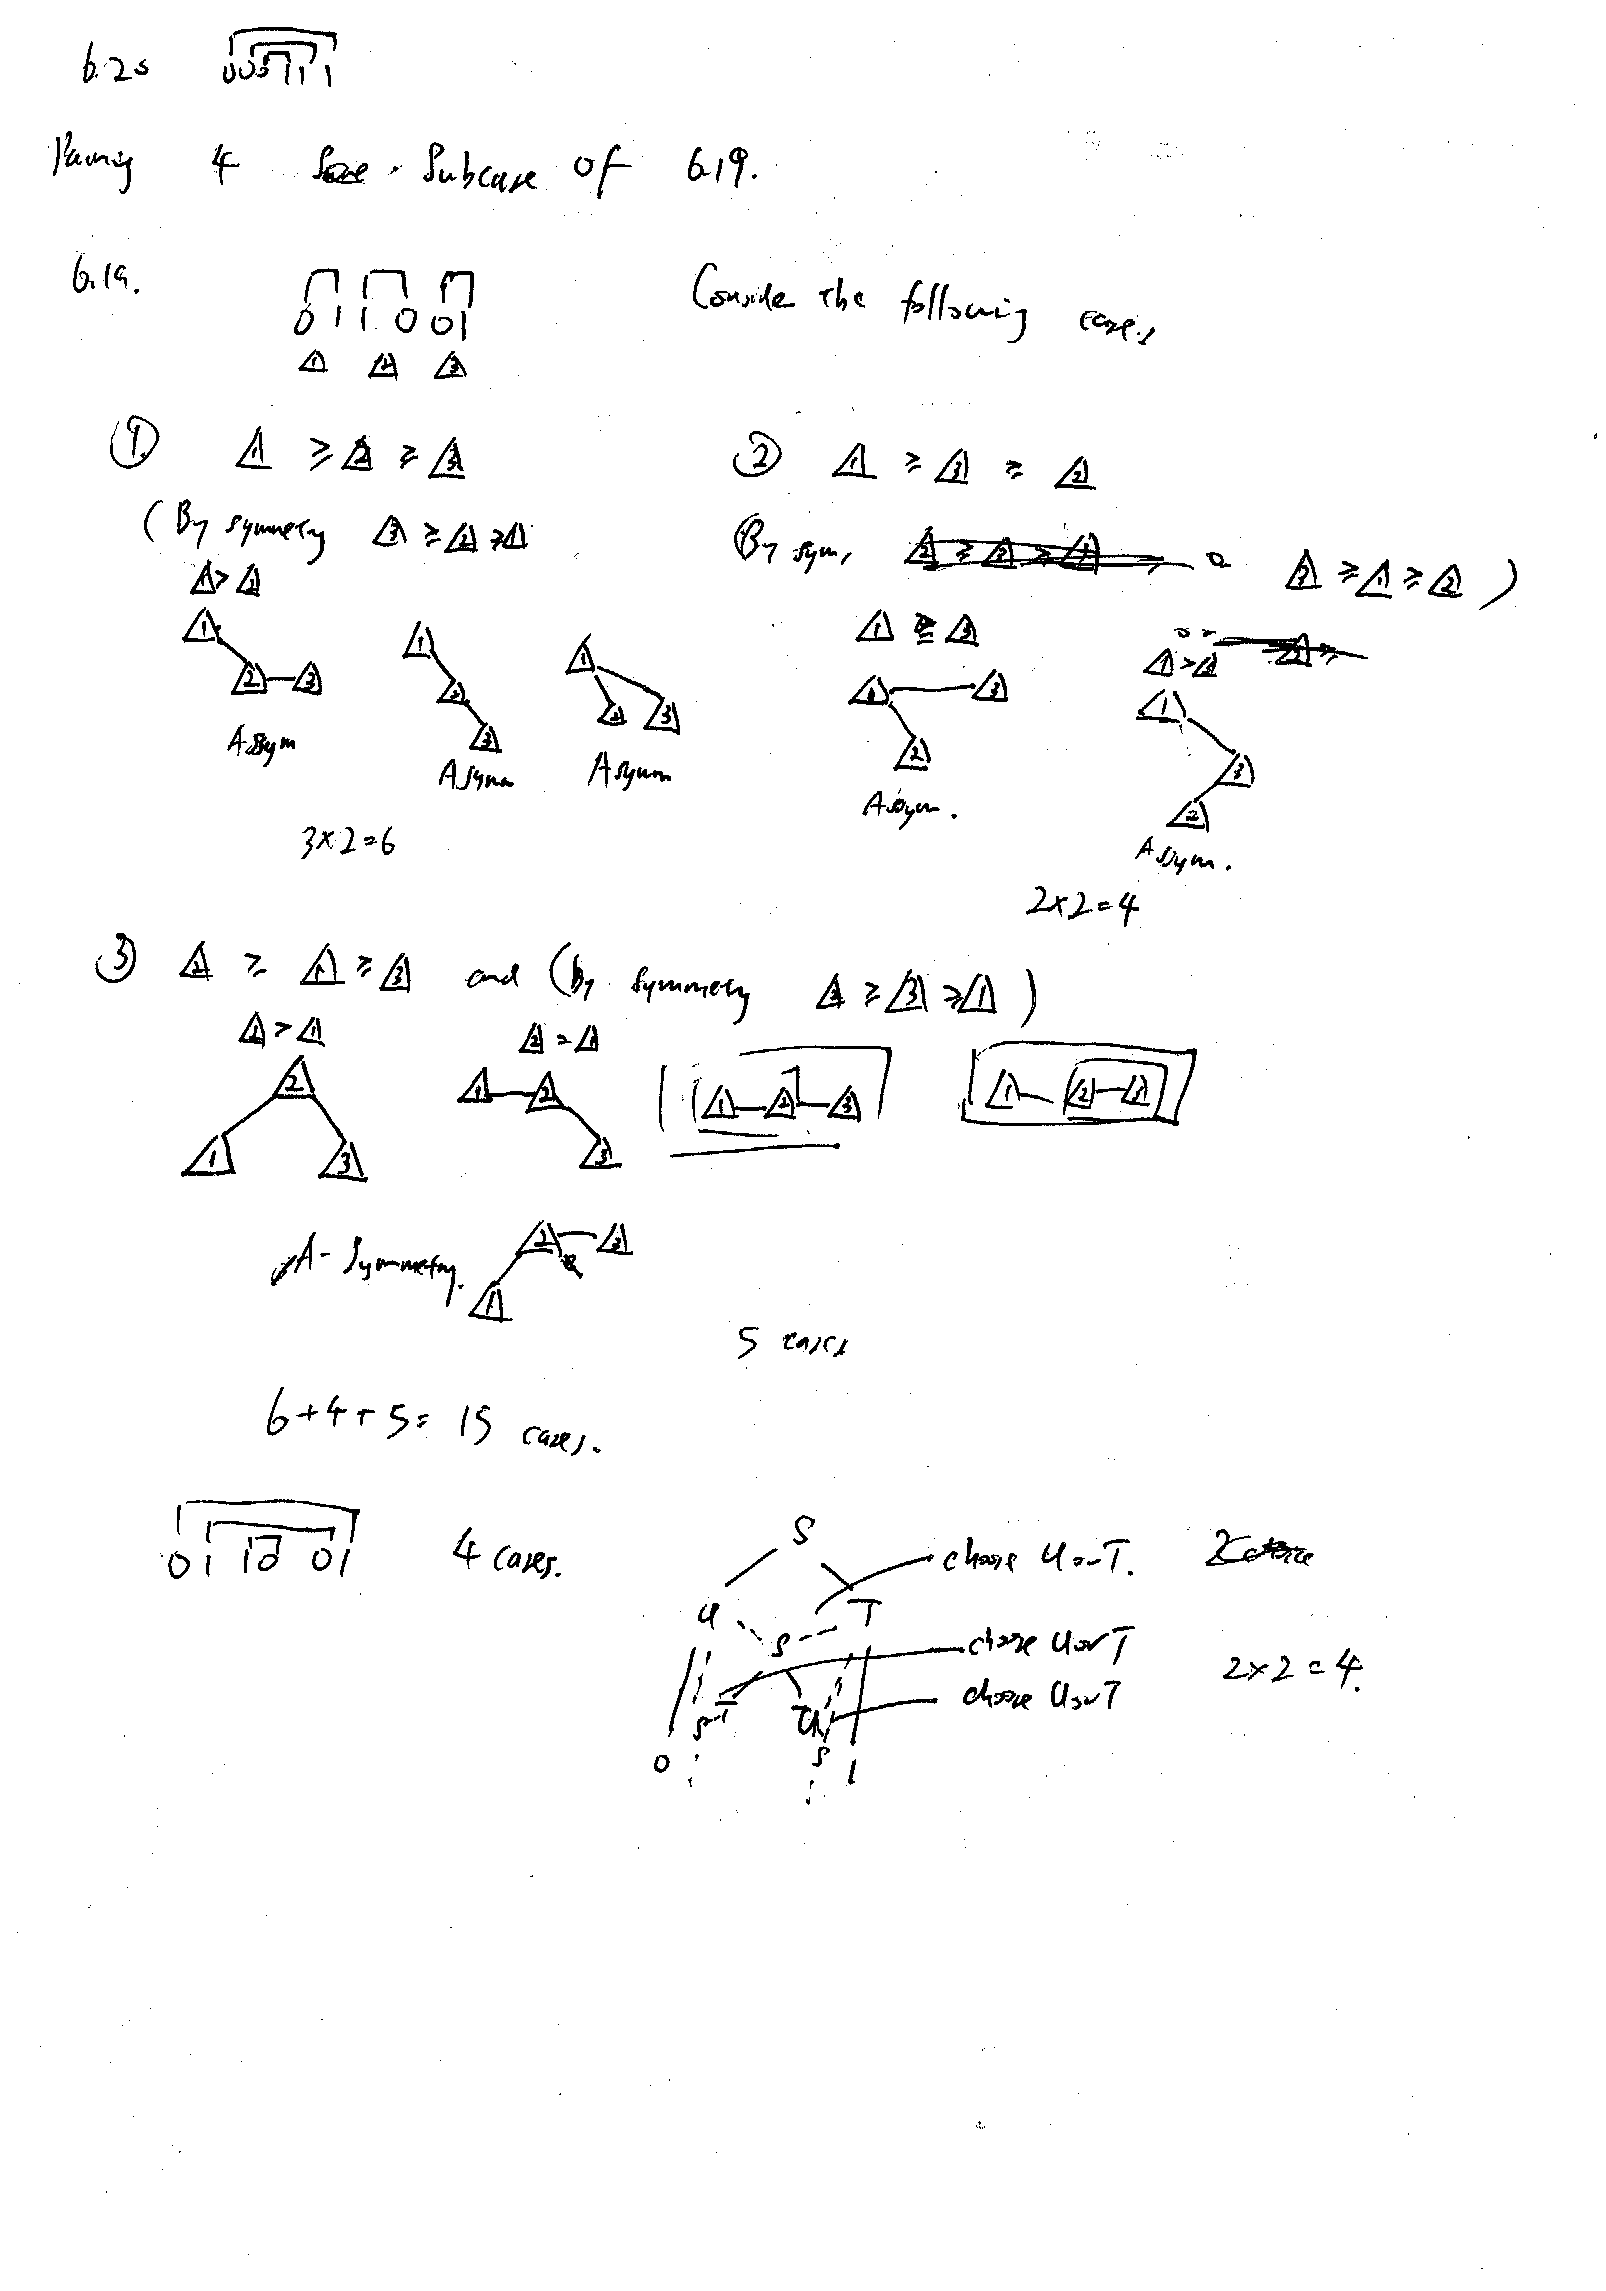
\includegraphics[scale=0.9]{qn6_19}


\paragraph{6.4}
\begin{align*}
	&(\{S,S_1,S_2,S_3,T,U,V,W\}, \{0,1\}, P, S)\\
	&T\rightarrow UV | UW\\
	&V\rightarrow TW\\
	&U\rightarrow 0\\
	&W\rightarrow 1\\
	&S\rightarrow \epsilon | TS_1 | UV | UW\\
	&S_1\rightarrow TS_2 | UV | UW\\
	&S_2\rightarrow TS_3 | UV | UW\\
	&S_3\rightarrow UV
\end{align*}
This can be simplified for e.g. by replacing $S_3$ with $T$.

Additional note: $T\rightarrow \epsilon$ cannot be added since it goes against Chomsky NF's requirements, instead, adding $T\rightarrow UW$ is actually equivalent, since the equivalent of $T$ generating $\epsilon$, is to simply generate fewer $T$'s.

\paragraph{6.5}
\begin{align*}
	U&\rightarrow 0\\
	W&\rightarrow 1\\
	V&\rightarrow TW\\
	T&\rightarrow UW|UV\\
	S&\rightarrow UW|UV|ST\\
	S'&\rightarrow UW|UV|ST
\end{align*}

\paragraph{6.6}
\begin{align*}
	U&\rightarrow 0\\
	V&\rightarrow 1\\
	S&\rightarrow US_1\\
	S_1&\rightarrow VS_2\\
	S_2&\rightarrow VU\\
	S&\rightarrow UT_1\\
	T_1&\rightarrow ST_2\\
	T_2&\rightarrow ST_3\\
	T_3&\rightarrow VT_4\\
	T_4&\rightarrow VT_5\\
	T_5&\rightarrow ST_6\\
	T_6&\rightarrow SU\\
	S'&\rightarrow US_1 | UT_1
\end{align*}
\pagebreak

\paragraph{7.11}
L is not linear. By elimination, H, K must be linear.

A linear grammar for H is as follows.
\begin{align*}
	S \rightarrow 0S2 | 1S2 | \epsilon
\end{align*}

A linear grammar for K is as follows
\begin{align*}
	S \rightarrow S_1 | S_2\\
	S_1\rightarrow S_12 | T_1 | T_2\\
	S_2\rightarrow 0S_2 | T_3 | T_4\\
	T_1\rightarrow 1 | T_11 | 0T_11\\
	T_2\rightarrow 0 | 0T_2 | 0T_21\\
	T_3\rightarrow 2 | T_32 | 1T_32\\
	T_4\rightarrow 1 | 1T_4 | 1T_42
\end{align*}
Reasoning for K, 
\begin{itemize}
	\item $S_1: n\neq m$
	\item $S_2: m\neq k$
	\item $T_1: n<m$. To be precise, $T_1$ generates $\{0^n1^m:n<m\}$.
	\item $T_2: n>m$
	\item $T_3: m<k$
	\item $T_4: m>k$
\end{itemize}




\paragraph{7.18} We count the derivation tree as follows. Since $(W,132)$ is non-zero at the tree root, we can have 132 derivation trees of 0000111.

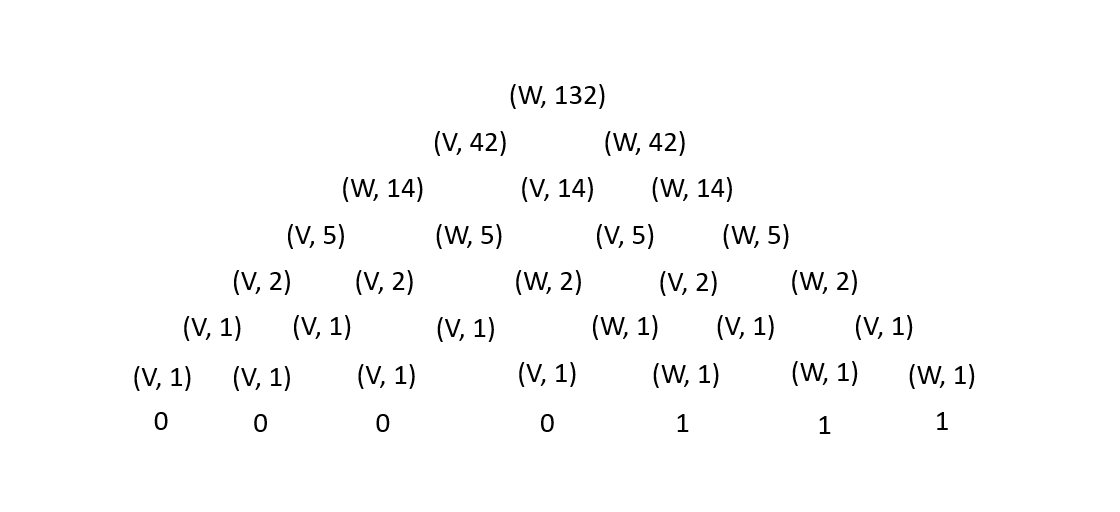
\includegraphics[scale=0.7]{qn7_18}

\paragraph{7.23} Proof by induction on n.

We need to show $(k-1)^{n+1} - 1\leq k^n(k-2)$.

For instance, the base case where $n = 1$, is shown by $(k-1)^2 - 1 = k^2 - 2k +1 - 1 = k^2 - 2k = k(k-2)\leq k(k-2)$.

Alternatively by binomial expansion, we get
\begin{align*}
	k^n = (k-1 + 1)^n = \sum_{0\leq i\leq n}\binom{n}{i} (k-1)^i \geq \sum_{0\leq i\leq n}(k-1)^i = (k-1)^{n+1} - 1
\end{align*}

\paragraph{7.24}
The algorithm is very similar, but instead of returning 1 or 0, the algo returns the length of the shortest derivation.\\
Note that Min refers to the algo, whereas min is the mathematical set operation.
\begin{align*}
	Min(u,v,t) := \min(\{Min(u,u',t') + Min(u',v,t') : u'\in (N\cup \Sigma)^*, |u|\leq |u'|\leq |v| \}\cup \{\infty \})
\end{align*}
where $t'$ is similarly defined as in $Check(u,v,t)$

\paragraph{Example 7.28} Let $L$ be an infinite language satisfying lemma 2.15(b) with pumping constant $k$. We let $c=2k$ and claim that for any $t\in \mathbb{N}$, we can find a word $u\in L$ such that $|u|\in \{t, t+1, \dots, t+c\}$

For any word $u$, $|u|\geq k$, we can always pump it down until it's length $l$ is $k\leq l< 2k$. Hence, WLOG, we assume that $k\leq |u|<2k$. This also implies that for each $t\in \{0, \dots, |u|\}, |u| \in \{t, t+1, \dots, t+c\}$.

Now since $|u|\geq k$, there is a splitting $u=vwxyz$ such that $\forall h\in \mathbb{N}, vw^hxy^hz\in L$. We note that the difference between adjacent words, $|vw^{h+1}xy^{h+1}z| - |vw^hxy^hz|=|wy|\leq k$, such that $\forall \lambda \in \mathbb{N}$, there is a word in $L$ of length $|w|+\lambda |bd|$.

Now let $t>|w|$. We can find $\lambda$ such that $|w|+\lambda |bd|\leq t<|w|+(\lambda + 1)|bd|\leq t+k < t+c$. In particular, $|w|+(\lambda + 1)|bd|\in \{t, t+1, \dots, t+c\}$.

And we are done with the proof.

\paragraph{7.29} Let $L$ be such a context free language and $G$ a context free grammar generating $L$.

Convert $G$ to $G'$ in Chomsky Normal Form, where $G'=(N', \Sigma, P', S')$. We now construct $G''=(N'', \Sigma, P'', S'')$ in the following manner.

$S'' = S'$\\
Define rules $P''$ as follows. (We add elements into $N''$ as required by the rules).\\
We first add all rules $A\rightarrow BC\in P'$ into $P''$.\\
For all rules of form $A\rightarrow BC$, if $B\rightarrow b$, add the rule $A\rightarrow bC$ into $P''$.
If $C\rightarrow c \in P'$, add the rule $A\rightarrow Bc$ into $P''$.\\
If $B\rightarrow b\in P'\land C\rightarrow c \in P'$, add the rule $A\rightarrow bc$ into $P''$.

Then $G''$ generates all words with length $>1$ in $L$.

Hence $L = H_1\cup H_2$, where $H_1$ is the language generated by $G''$ and \\
$H_2=\{a\in \Sigma : a\in L\}$ if $\epsilon \notin L$,\\
$H_2=\{a\in \Sigma : a\in L\}\cup \{\epsilon \}$ if $\epsilon \in L$.

\paragraph{7.30} Let $G = (N, \Sigma, P, S)$ be a grammar. We will construct a corresponding growing context sensitive grammar $G' = (N', \Sigma', P', S')$

\begin{itemize}
	\item $S' = S$
	\item $N' = N$
	\item $\Sigma' = \Sigma \cup \{0\}$, where $0$ is not a symbol in $\Sigma$
	\item For each rule $l\rightarrow r \in P$, add the rule $l\rightarrow r0^{|l| + 1}$. This is so that $|RHS| = |r| + |l| + 1\geq |l|+1 > |l|$, hence the new grammar is growing.
	\item Homomorphism $h$ such that $\forall i\in \Sigma \cup N, h(i) = i$ and $h(0) = \epsilon$.
\end{itemize}

\paragraph{Designing PDAs}
There are a few common tricks to make designing PDAs easier.
\begin{itemize}
	\item Make generous use of $\epsilon$-transitions, especially if the PDA is not required to be deterministic. An epsilon transition is a transition in which no input is read. e.g. $\delta(q, v, A)$ where $v=\epsilon$. This can greatly reduce the number of cases to consider.
	\item There are 2 general ways to enforce the following inequality. To be precise, I use this example: We want to check for $0^n1^m$, where $n\leq m+k$ for some fixed $k>0$.
	\begin{itemize}
		\item One way is to push $k$ extra \textbf{non-terminals} in a single shot.
		\item The other way is to have $k$ extra intermediate \textbf{states} that consume the non-terminals generated by parsing $0$'s.
	\end{itemize}
\end{itemize}

\paragraph{8.9}\mbox{}

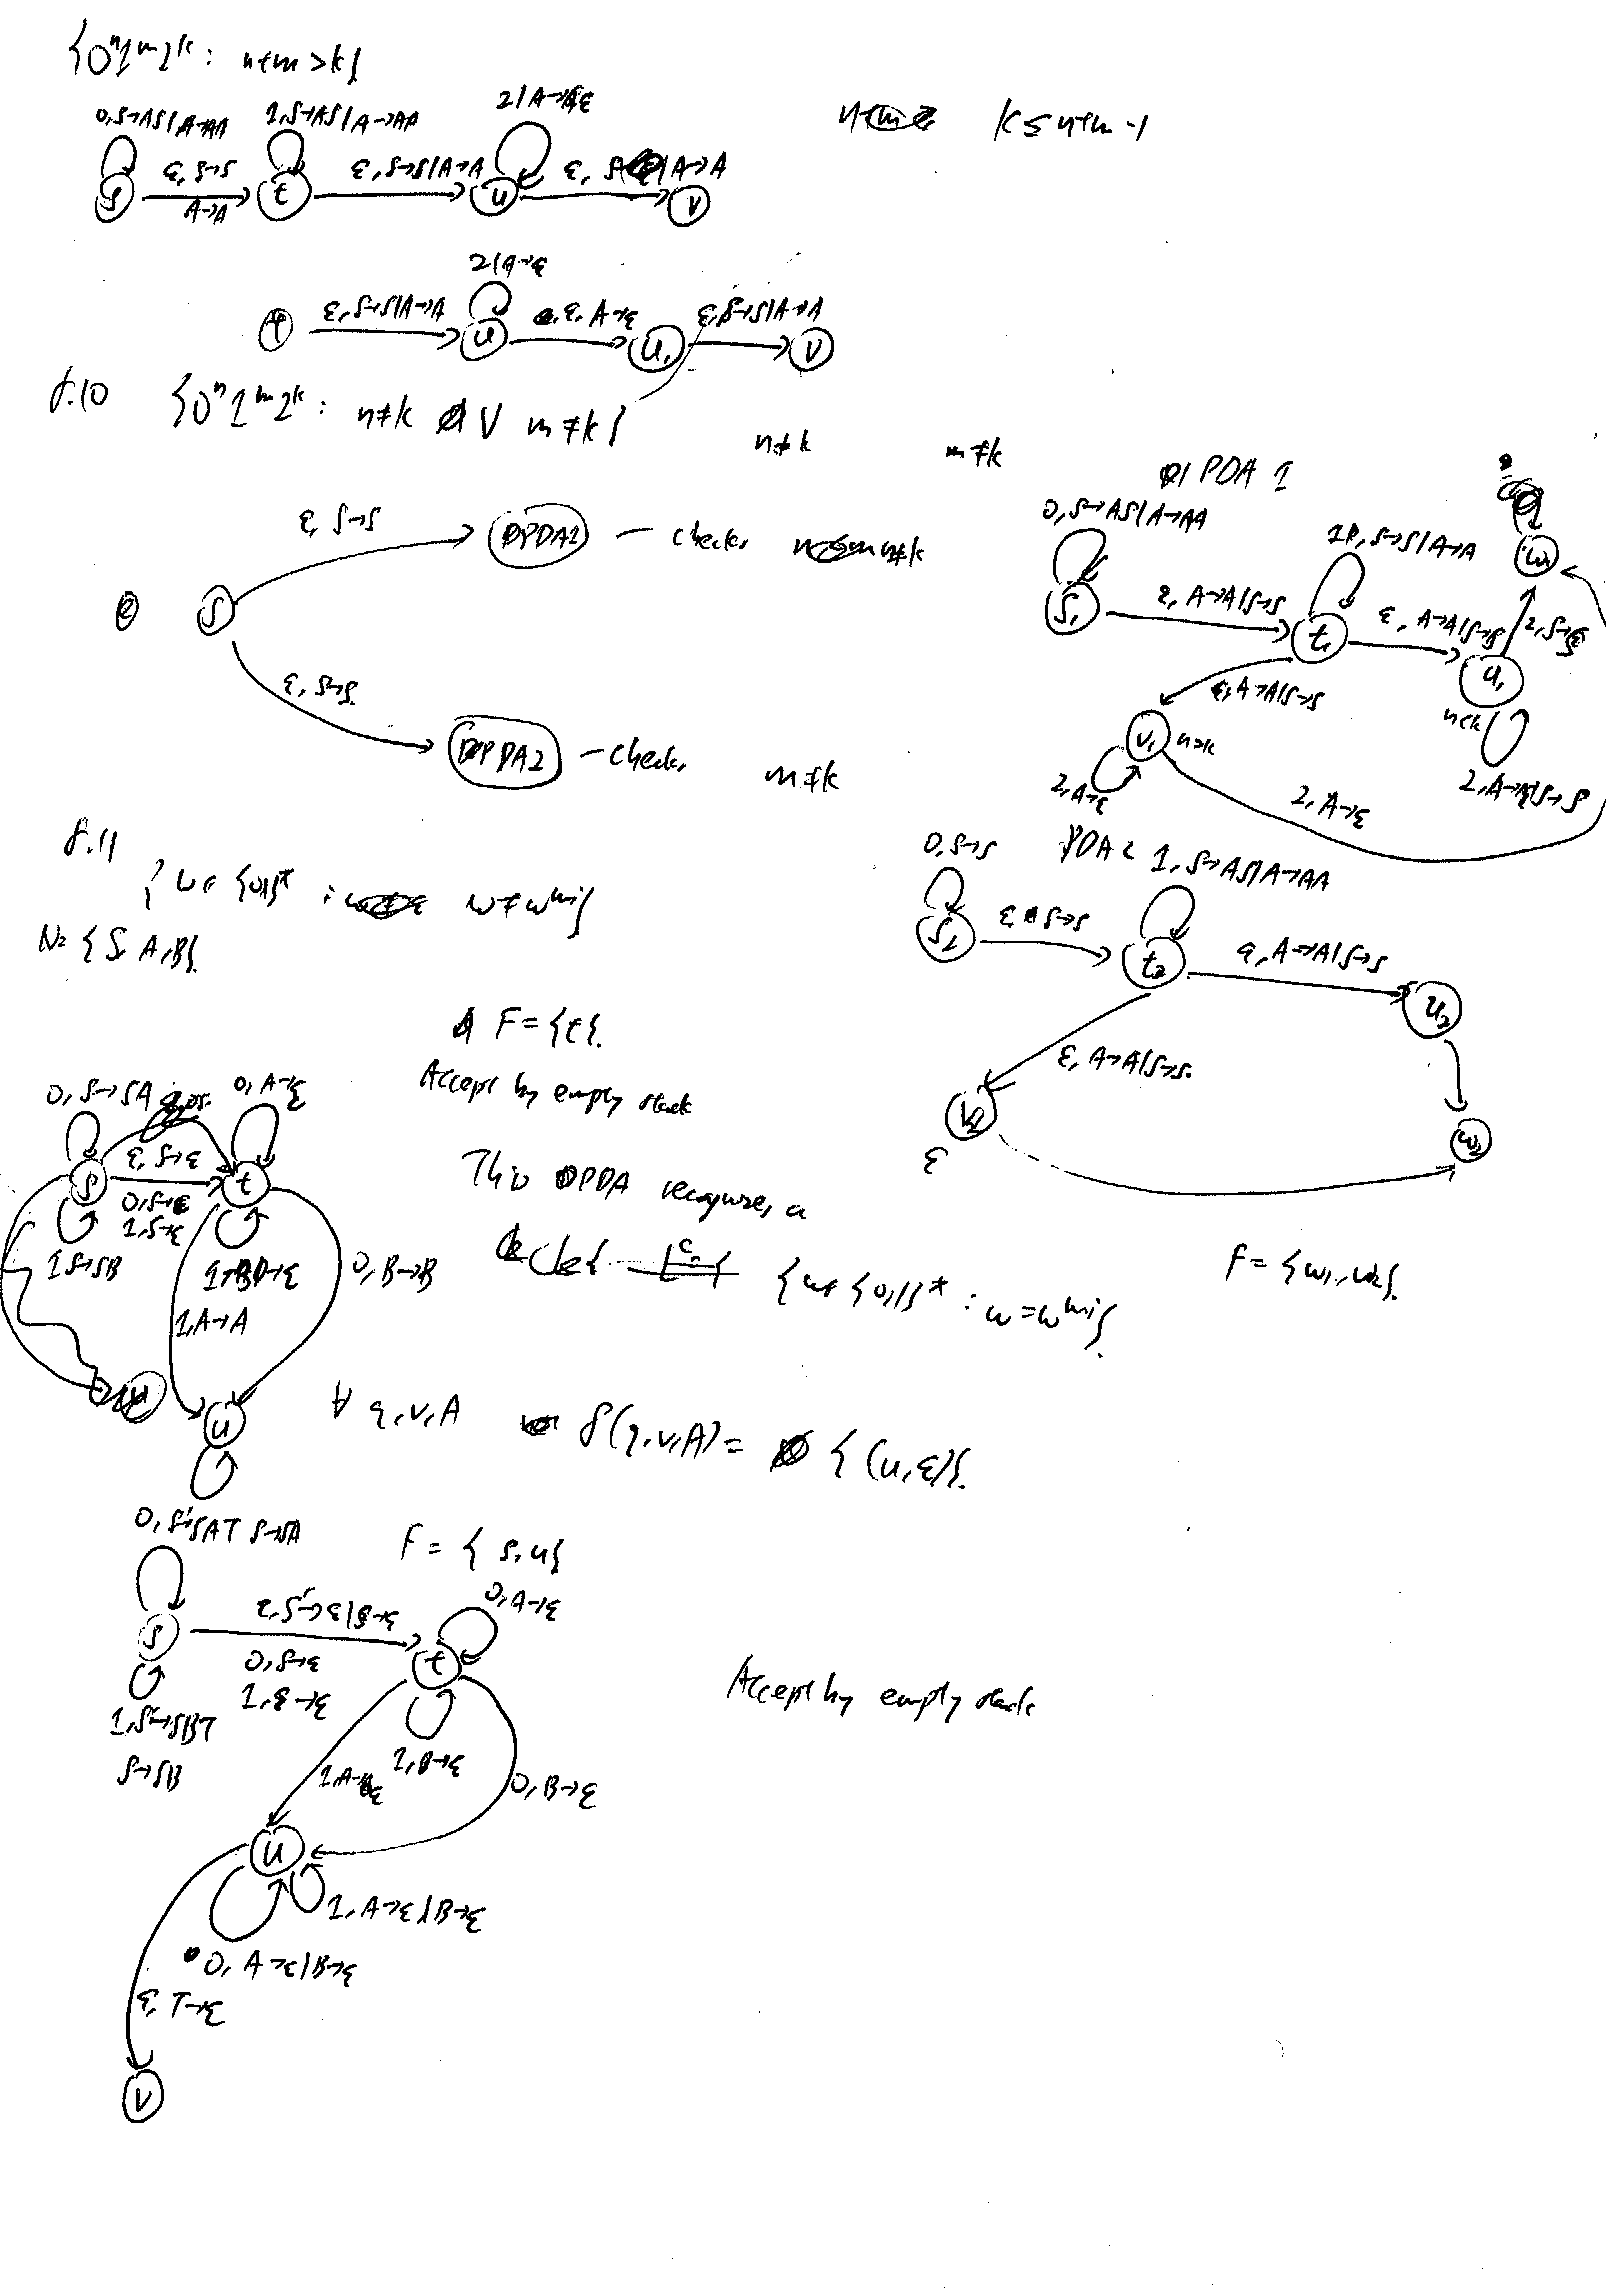
\includegraphics[scale=0.7]{q8_9}

\paragraph{Example 8.17} We will prove that $\forall w\in L, ds(w) < |w|$, where $ds(w)$ denotes the digit sum of $w$.

We will conduct induction on derivation length. For brevity, we skip the base case. Our induction hypothesis is that for all words $w$ that can be derived via a derivation of length $\leq n$, we must have $ds(w) < |w|$.

Now let $w\in L$ be a word for which there exists a derivation of length $n+1$. We consider the first step of such a derivation.

\begin{itemize}
	\item Case 1: $S\Rightarrow 0$. Then $w=0$ and we clearly have $ds(w) = 0 < 1 = |w|$
	\item Case 2: $S\Rightarrow 1S\Rightarrow^* 1v$, where $S\Rightarrow^* v$ takes $n$ steps and $w=1v$. By the induction hypothesis, $ds(v) < v$. Hence $ds(w) = 1 + ds(v) < 1 + |v| = |w|$
	\item For the other 2 cases, we note that the induction hypothesis, $ds(v) < |v|\implies ds(v)\leq |v|-1$.\\
	Case 3: $S\Rightarrow 2SS\Rightarrow^* 2v_1v_2$, where $SS\Rightarrow^* v_1v_2$ in $n$ steps. By our induction hypothesis, we have $ds(w) = 2 + ds(v_1) + ds(v_2) \leq |v_1| + |v_2| = |w| - 1 < |w|$\\
	The final case where $S\Rightarrow 3SSS\Rightarrow^* 3v_1v_2v_3$ is similarly proven.
\end{itemize}

\paragraph{Proposition 8.20} Note that another consequence of this theorem is that given a DPDA, we can construct an equivalent DPDA recognizing the same language that does not get stuck.

\paragraph{8.24}
We first construct a context free grammar for the language $L=\{0^n10^m : n\geq m\}$.

\begin{itemize}
	\item $S\rightarrow 0SV_0 | 1$
	\item $V_0\rightarrow 0 | \epsilon$
\end{itemize}

The deterministic pushdown automaton is defined as follows. Note that a dpa is allowed to get stuck. Also, a dpa must accept by state.

\begin{itemize}
	\item $Q=\{s,t\}$
	\item $F=\{t\}$
	\item $N=\{S, V_0\}$
	\item $\Sigma = \{0,1\}$
\end{itemize}

\begin{align*}
	\delta(s,0,S) = \{(s, SV_0)\}\\
	\delta(s,1,S) = \{(t,\epsilon)\}\\
	\delta(s,0,V_0) = \{(t,\epsilon)\}\\
	\delta(s,\epsilon,V_0) = \{(t,\epsilon)\}
\end{align*}

The dpa gets stuck when all the $V_0$ in the stack are consumed, but the state at this point must be $t$.


We first suppose that $L^*$ is DCFL. Recall the DCFLs are closed under complement and closed under union and intersection with regular languages.

Hence, $H:=(L^*\cap 0^*10^*) \cup (L^*\cap 0^*10^*10^*) = \{0^a10^b : a\geq b\}\cup \{0^a10^b10^c : b\geq c\}$ must be DCFL.

Using a rewiring argument, we can show that $H$ is not DCFL. Let $M_1$ be a deterministic pushdown automatons recognizing $H$. We conduct the rewiring as follows:

$M_2$ is a DPDA recognizing the language $H'$ formed by replacing all 0s with 2s.

We connect the accepting states of $M_1$ for $\{0^a10^b : a\geq b\}$ (and change them to rejecting) to the states of $M_2$ that are "halfway" to the accepting states of $\{2^a12^b12^c : b\geq c\}$. The resulting DPDA then accepts a certain language $L$ that has $\{0^a10^b12^c : a\geq b\geq c\}$ as a subset. Note that $L$ does not have any other elements of the form $0^a10^b12^c$.

$L$ is not context free as it fails the pumping lemma 2.15(b). Hence we arrive at a contradiction and $L^*$ is not deterministic context free.
 
 
\paragraph{8.25} We are given that $L$ is DCFL and $H$ is a regular language. Claim: $L\cdot H$ is DCFL.

Let $(Q, \Sigma, N, \delta, s, S, F)$ be a DPDA for $L$.\\
Let $(Q', \Sigma, \delta', s', F')$ be a DFA for $H$.\\

Consider the following DPDA.
\begin{align*}
	(Q\times \mathcal{P}(Q'), \Sigma, N, \delta'', s'', S, F'')
\end{align*}
where
\begin{align*}
s''&=
\begin{cases}
(s, \emptyset) \text{ if }\epsilon \notin L\\
(s, \{s'\} \text{ if }\epsilon \in L
\end{cases}
\\
\delta''((q, q''), \epsilon, A)&=
\begin{cases}
\{((p, q''), w) : (p, w)\in \delta(q, \epsilon, A)\} \text{ if }p\notin F\\
\{((p, q'' \cup \{s'\}), w) : (p, w)\in \delta(q, \epsilon, A)\} \text{ if }p\in F
\end{cases}
\\
\delta''((q, q''), a, A)&=
\begin{cases}
\{((p, \{\delta'(q') : q'\in q''\}), w) : (p, w)\in \delta(q, a, A)\} \text{ if }p\notin F\\
\{((p, \{\delta'(q') : q'\in q''\} \cup \{s'\}), w) : (p, w)\in \delta(q, a, A)\} \text{ if }p\in F
\end{cases}
\\
F''&=\{(q, q'') : q''\cap F'\neq \emptyset\}
\end{align*}

This DPDA recognizes $L\cdot H$. Hence $L\cdot H$ is a DCFL.

\paragraph{8.26} Given that $L$ is DCFL and $H$ is regular, is $H\cdot L$ DCFL?

The general idea of the counterexample is as follows. Let's say we have 2 DCFL languages $L_1, L_2$, such that we know very well that $L_1\cup L_2$ is not DCFL. Now how do we make use of this?

Suppose $L_1, L_2\subseteq \Sigma^*$. We find some letter $a\notin \Sigma^*$. And it is quite easy to see that $a\cdot L_1\cup L_2$ is DCFL. Why? Because we know that there exists a DPDA $M_1$ recognizing $L_1$, and a DPDA $M_2$ recognizing $L_2$. We can combine these two DPDA to form a DPDA $M$ that does the following: Check the first letter of the input. If the first letter is $a$, since we know that $a\notin \Sigma$, we must be dealing with $L_1$, otherwise if the first letter is in $\Sigma$, then we must be dealing with $L_2$. So, if the first letter is $a$, $M$ delegates the work to $M_1$, and otherwise, $M$ delegates the work to $M_2$.

Here, we suppose that left concatenation of a regular language to a DCFL results in a DCFL (in order to arrive at a contradiction).\\
Then in particular, $a^*\cdot (a\cdot L_1\cup L_2)$ is a DCFL.\\
Since DCFLs are closed under intersection with regular languages, 
\begin{align*}
	(a^*\cdot (a\cdot L_1\cup L_2)) \bigcap (a\cdot \Sigma^*) = a\cdot L_1 \cup a\cdot L_2
\end{align*} must be DCFL.
But now the first $a$ is meaningless. Intuitively, it tells nothing about whether a word is about to be in $L_1$ or $L_2$. Hence, $L_1\cup L_2$ must be DCFL, a contradiction.

An example of such $L_1, L_2$ would be the following:
\begin{align*}
	L_1 = \{0^n1^n : n\in \mathbb{N}\}\\
	L_2 = \{0^n1^{2n} : n\in \mathbb{N}\}\\
	L_1\cup L_2 = \{0^n1^n, 0^n1^{2n} : n\in \mathbb{N}\}
\end{align*}
A rewiring argument can be used to show that $\{0^n1^n, 0^n1^{2n} : n\in \mathbb{N}\}$ is not a DCFL.

This also works when we know of 2 DCFL whose intersection is not a DCFL. Suppose we have $L_1, L_2$ DCFL, but $L_1\cap L_2$ not a DCFL. Then since DCFL are closed under complement, $(L_1\cap L_2)^c = L_1^c\cup L_2^c$ is not a DCFL, even though $L_1^c,L_2^c$ are DCFLs. An example of such languages would be $L_{0,1}$ and $L_{1,2}$ introduced in the textbook. $L_{0,1}$ is the set of all words with as many 0s as 1s. $L_{1,2}$ is the set of all words with as many 1s as 2s.

\paragraph{8.29}
The answer is YES.
If one has a language $H_k$, one looks at the derivative which comes along b. So for each $H_k$, one makes a nonterminal $X_k$. Now if $H_k$ derived by b gives $H_i H_j H_h$ (or any other product) then one makes the rule $X_k -> b X_i X_j X_h$. Here are some specific cases. If $H_k$ derived b gives {epsilong} then the rule is just $X_k -> b$. If $H_k$ derived b gives emptyset then there is no rule (or a rule $X_k -> b X_3$ where $H_3$ is the emptyset.
Start symbol is $X_1$ which represents $H_1 = L$.

This condition to be added is sufficient and Exercise 8.30 shows that without this condition, one cannot make the grammar. Indeed, it is an “if and only if” condition.



\paragraph{8.32}
\begin{align*}
	(L\cup H)_x &= \{w\in \Sigma^* : xw\in L\cup H\}\\
	&= \{w\in \Sigma^* : xw\in L\lor xw\in H\}\\
	&= \{w\in \Sigma^* : xw\in L\}\cup \{w\in \Sigma^* : xw\in H\}\\
	&= L_x\cup H_x
\end{align*}

\paragraph{9.3} Construct a Turing machine representing the function $x\mapsto 3x$. We consider the following machine with state $Q=\{s,t,u,v,w\}$.
\begin{itemize}
	\item $s$ is the start state when the Turing machine scans the word from left to right.
	\item $t,u,v$ are the states where the Turing machine actually does processing
	\item We note that $3x=x+2x$. With this in mind, if we let $x=b_nb_{n-1}\dots b_0$, to get $3x$, we need to add $0b_nb_{n-1}\dots b_0$(x) and $b_nb_{n-1}\dots b_00$(2x). At any point in time, we are adding three bits, the carry bit $C$, the "previous bit" $b_{i-1}$ and the current bit $b_{i}$. To account for the edge cases, we take $b_{-1}=0$ and $b_{n+1}=0$.
	\begin{itemize}
		\item $t$ represents having $C+b_i=0$
		\item $u$ represents having $C+b_i=1$
		\item $v$ represents having $C+b_i=2$
	\end{itemize}
	\item $w$ is the halting state, i.e. $F=\{w\}$
\end{itemize}
The rules are as follows:
\begin{align*}
	\delta(s,0)&=(s,0,\rightarrow)\\
	\delta(s,1)&=(s,1,\rightarrow)\\
	\delta(s,\sqcup)&=(t,\sqcup,\leftarrow)\\
	\delta(t,0)&=(t,0,\leftarrow)\\
	\delta(t,1)&=(u,1,\leftarrow)\\
	\delta(u,0)&=(t,1,\leftarrow)\\
	\delta(u,1)&=(v,1,\leftarrow)\\
	\delta(v,0)&=(u,0,\leftarrow)\\
	\delta(v,1)&=(v,1,\leftarrow)\\
	\delta(t,\sqcup)&=(w,\sqcup,\leftarrow)\\
	\delta(u,\sqcup)&=(w,1,\leftarrow)\\
	\delta(v,\sqcup)&=(u,0,\leftarrow)
\end{align*}

\paragraph{9.4} Construct a Turing machine representing the function $x\mapsto x+5$. We consider the following machine with state $Q=\{s,t_0,t_1,t_2,t_1',t_2',t,u\}$.

We are trying to add $x$ to $(101)_2$, the binary representation of $5$. In order to track the position of the word we are reading, we need the extra states $t_0$ to $t_2$. The primed states $t_1'$ and $t_2'$ representing having a carry bit of $1$.

$u$ represents having a carry bit of $1$, $t$ represents having a carry bit of $0$ (i.e. no carry).

\begin{align*}
	\delta(s,0)&=(s,0,\rightarrow)\\
	\delta(s,1)&=(s,1,\rightarrow)\\
	\delta(s,\sqcup)&=(t_0,\sqcup,\leftarrow)\\
	\delta(t_0,0)&=(t_1,1,\leftarrow)\\
	\delta(t_0,1)&=(t_1',0,\leftarrow)\\
	\delta(t_1,0)&=(t_2,0,\leftarrow)\\
	\delta(t_1,1)&=(t_2,1,\leftarrow)\\
	\delta(t_1',0)&=(t_2,1,\leftarrow)\\
	\delta(t_1',1)&=(t_2',0,\leftarrow)\\
	\delta(t_2,0)&=(t,1,\leftarrow)\\
	\delta(t_2,1)&=(u,0,\leftarrow)\\
	\delta(t_2',0)&=(u,0,\leftarrow)\\
	\delta(t_2',1)&=(u,1,\leftarrow)\\
	\delta(u,0)&=(t,1,\leftarrow)\\
	\delta(u,1)&=(u,0,\rightarrow)\\
	\delta(u,\sqcup)&=(t,1,\leftarrow)
\end{align*}

We let $F=\{t\}$. Notice that when state $t$ is reached, we no longer need to modify any more bits of the word on the tape.



\paragraph{Description 9.11}\mbox{}

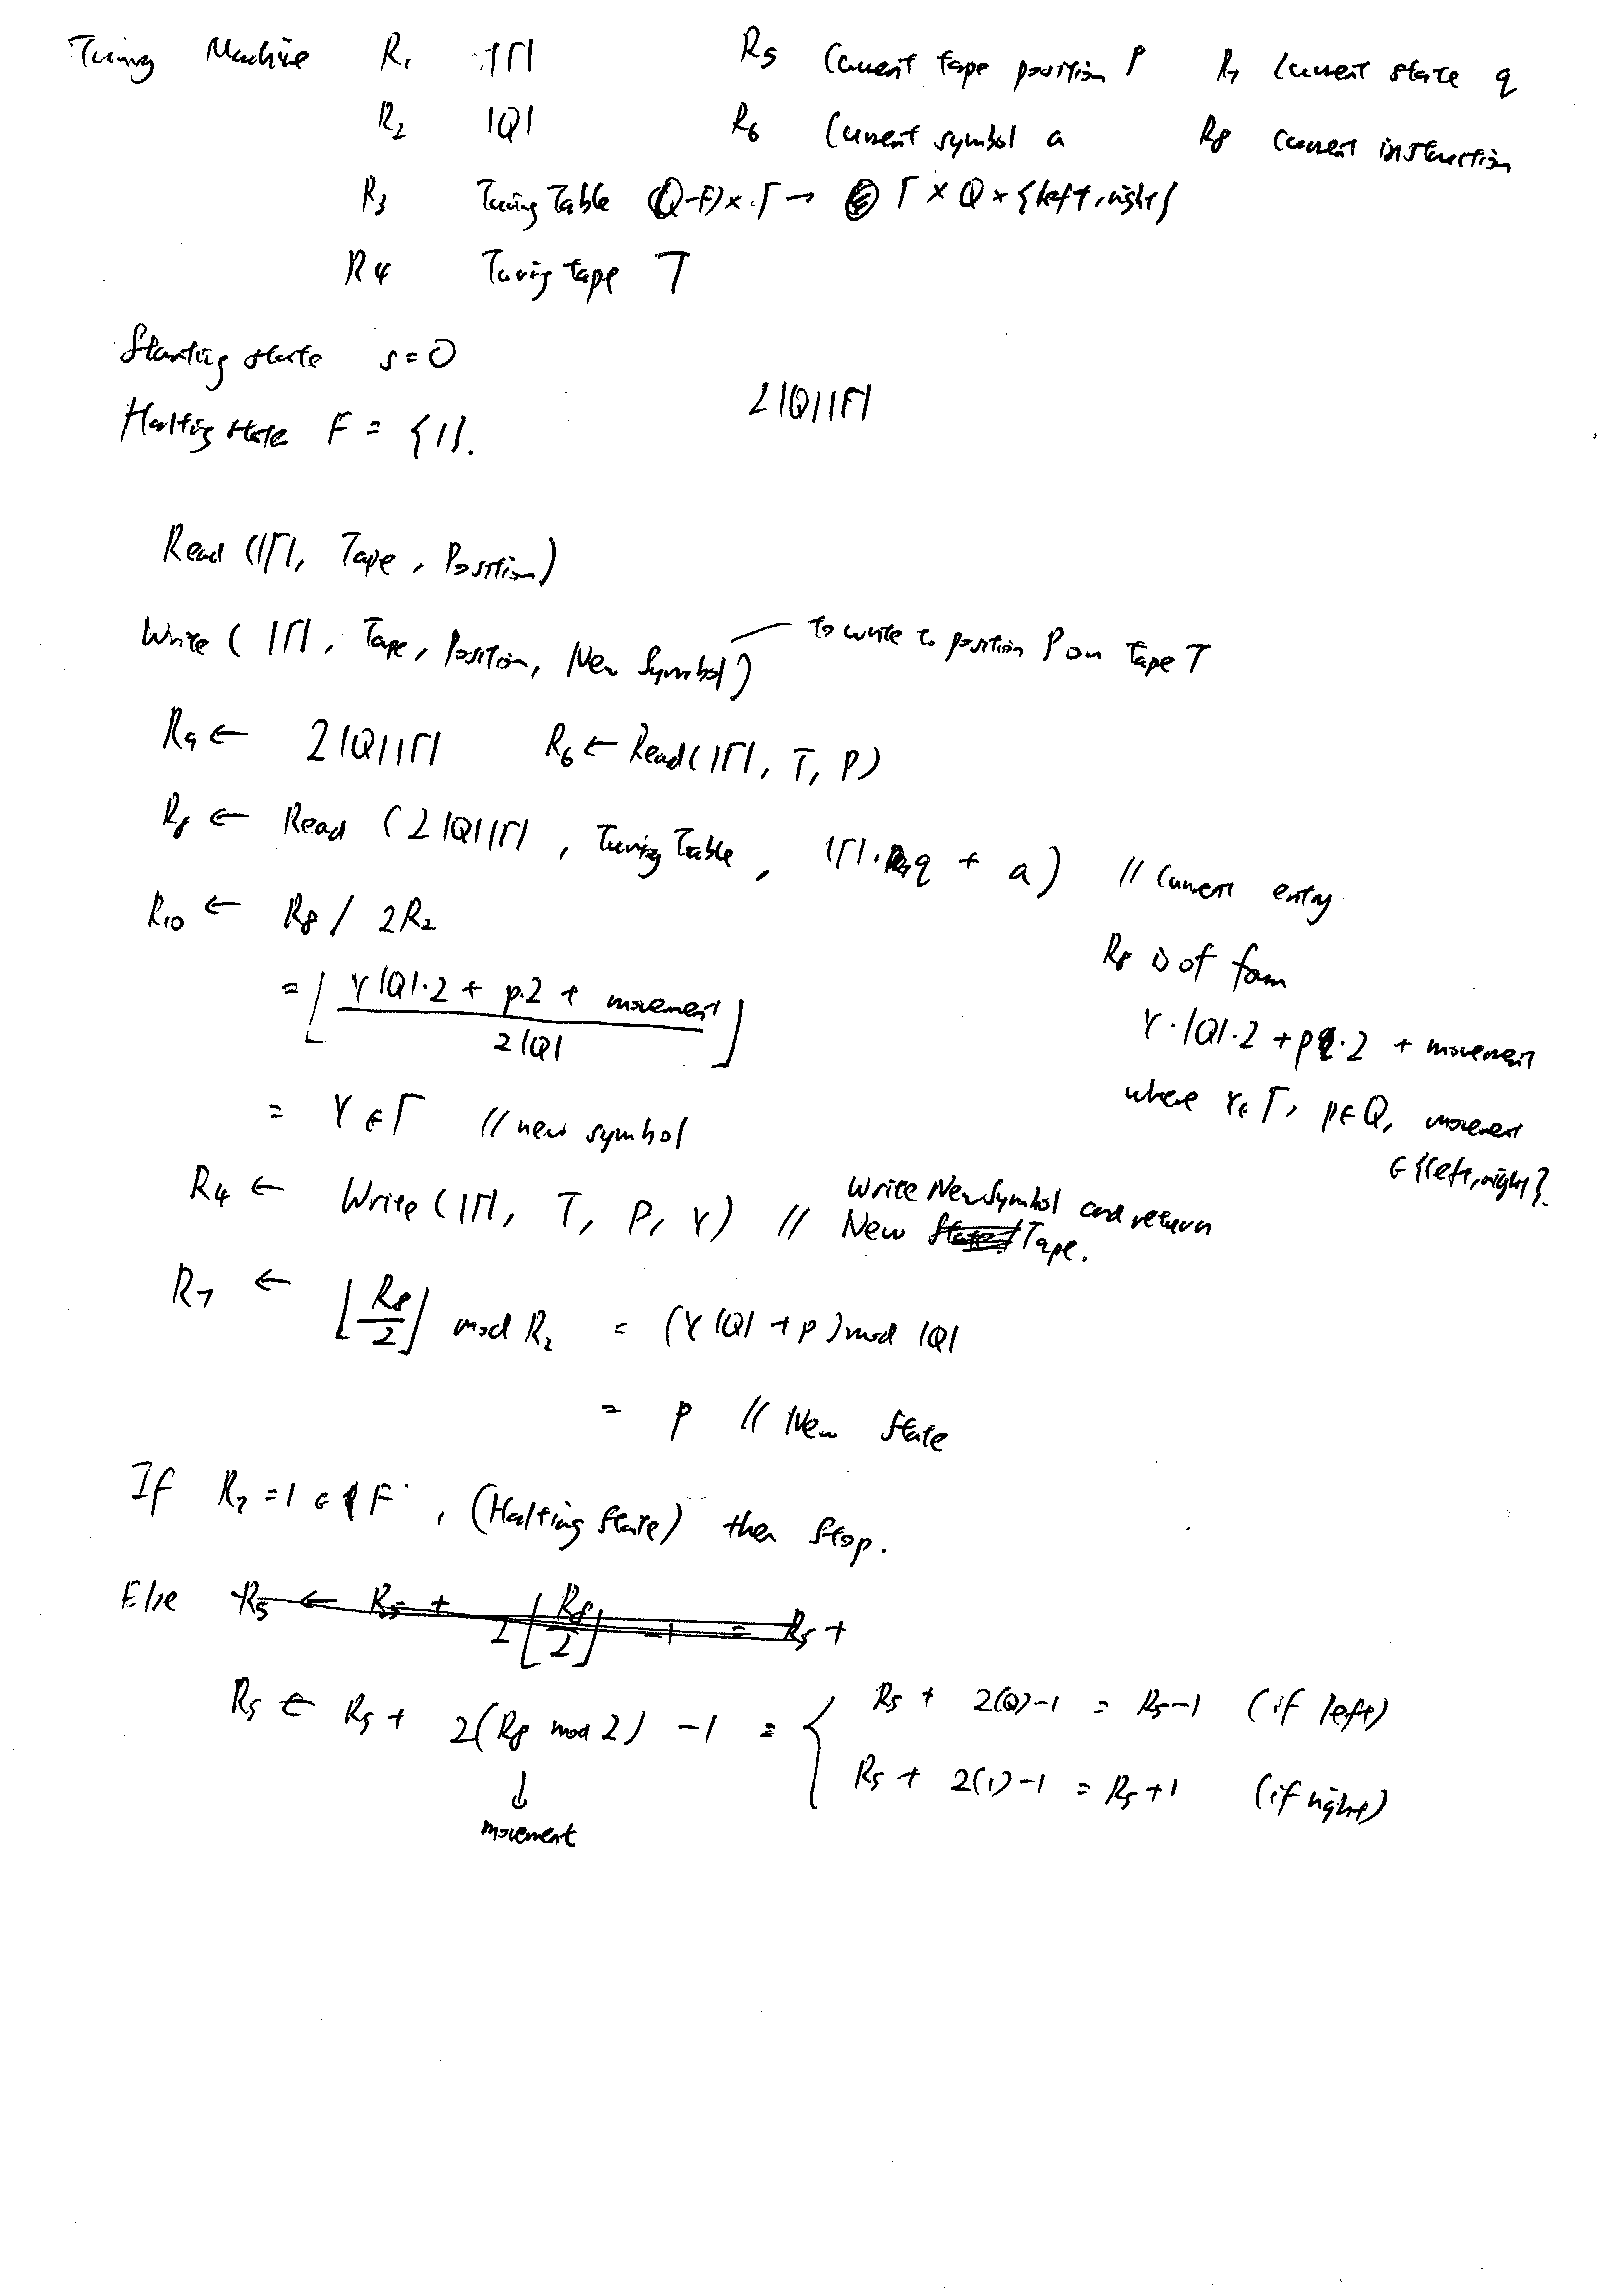
\includegraphics[scale=0.7]{9_11}

\paragraph{Example 9.17}\mbox{}
We define the following notations.
\begin{itemize}
	\item $Id: x\mapsto x$ is the identity function.
	\item $\phi_i: (x_1,x_2,\dots, x_n)\mapsto x_i$ is the projection function that selects the i-th entry. To be fully rigorous, we actually need to denote $\phi_i$ as $\phi_i^n$, since technically $\phi_i^n: (x_1,x_2,\dots, x_n)\mapsto x_i$ and $\phi_i^m: (x_1,x_2,\dots, x_m)\mapsto x_i$ are different functions accepting different inputs. However, we will be lazy and use $\phi_i$ when things are unambiguous. Also note that $Id=\phi_1^1$
	\item $\mathbf{0}$ as the constant zero function. Sometimes we will be lazy and not use boldface.
	\item $S:x\mapsto x+1$ or $succ:x\mapsto x+1$ as the successor function
	\item $P:x\mapsto x-1$ or $pred:x\mapsto x-1$ as the predecessor function. Note that $P(0)=0-1=0$.
\end{itemize}
Of the above function, $S$, $\phi_i$ are by definition, primitive recursive functions. Example 9.17 provides a proof that $P$ is a primitive recursive function as well.

Now we rewrite the examples in 9.17 in a more readable manner.

\textbf{Claim} $P$ is primitive recursive.\\
We use primitive recursion to define $P$.\\
$P(0):=f()=\mathbf{0}() = 0$, where $f=\mathbf{0}$\\
$P(x+1)=x:=g(x, P(x))$, where $g(x,y) = \phi_1(x,y)=x$\\
Hence, $P$ is primitive recursive.

\textbf{Claim} Addition, denoted by $h(x,y)=x+y$ is primitive recursive.\\
Like before, we use primitive recursion to define $h$.\\
$h(0,y):=f(y)=y$, where $f=Id$\\
$h(S(x),y):=g(x, h(x,y), y) = S(h(x,y))$, where $g(x,y,z)=S(y)=S(\phi_2(x,y,z))$. Note that $g$ is primitive recursive by composition.\\
Hence, $h$ is primitive recursive.

\textbf{Claim} Subtraction, denoted by $h'(y,x)=x-y$ is primitve recursive.\\
Using primitive recursion to define $h'$.\\
$h'(0,x):=f(x)=x$, where $f=Id$\\
$h'(S(y),x):=g(y,h'(y,x),x)=P(h'(y,x))$, where $g(x,y,z)=P(\phi_2(x,y,z))$.

\textbf{Corollary} $h(x,y)=x-y$ is primitive recursive.\\
Observe that $h(x,y)=h'(\phi_2(x,y),\phi_1(x,y))$, hence $h$ is primitive recursive by composition.


\textbf{Claim} Equality checking, denoted by $eq(x,y)=1-(x-y)-(y-x)$ is primitive recursive. (As before, $x-y=0$ if $x\leq y$)

Notice that $eq(x,y) = h(h(1, h(x,y)), h(y,x))$.\\
We first prove that $(x,y)\mapsto h(1, h(x,y))$ is primitive recursive. Note that the constant $\mathbf{1}$ function is primitive recursive. In fact, all constant functions are primitive recursive. Hence $(x,y)\mapsto h(1, h(x,y))$ can be viewed as a composition as follows: $h(\mathbf{1}(x,y), h(x,y))$. Hence $(x,y)\mapsto h(1, h(x,y))$ is primitive recursive.\\
We can use a similar composition argument for $eq$ itself, therefore $eq$ is primitive recursive.


\paragraph{9.18} Claim: Every function of the form $h(x_1,x_2,\dots,x_n)=\sum_{1\leq i\leq n}a_ix_i + b$ for some fixed $a_1,a_2,\dots,a_n,b\in \mathbb{N}$ is primitive recursive.

We will proceed by induction. For each $n\in \mathbb{N}$, let $P(n)$ be the statement that every function of the form $h(x_1,x_2,\dots,x_n)=\sum_{1\leq i\leq n}a_ix_i + b$ is primitive recursive.

We will show $P(0)$ as a base case. $P(0)$ essentially states that every constant function (with the constant being a natural number) is primitive recursive. We again proceed by induction and define for each $b\in \mathbb{N}$, the statement $Q(b)$ that the constant function $\mathbf{b}: any\mapsto b$ is primitive recursive. Clearly $Q(0)$ is true since $\mathbf{0}$ is a base case of the structural definition of primitive recursive functions. Now suppose $Q(b)$ true for some $b\in \mathbb{N}$. Then $\mathbf{b+1}=\mathbf{b}+\mathbf{1}=S(\mathbf{b})$, hence $\mathbf{b+1}$ is primitive recursive. This show $Q(b+1)$. Hence by induction, all constant functions are primitive recursive.

It is also easy to show that for any constant $a\in \mathbb{N}$, the function $x\mapsto x+a$ is primitive recursive. Because, for $a>1$, such a function involves repeated applications of the successor function $S$. So we take this fact for granted.

Let $n\in \mathbb{N}$ and suppose $P(n)$ true. Then
\begin{align*}
	h(x_1,x_2,\dots,x_{n+1})=\sum_{1\leq i\leq n+1}a_ix_i + b = a_1x_1 + \sum_{2\leq i\leq n+1}a_ix_i + b
\end{align*}

We now attempt to define $h$ using the recursive strategy.

When $x_1=0$, we have $h(0, x_2, \dots, x_{n+1}) = h'(x_2,\dots, x_{n+1})$, where $h'(y_1, y_2,\dots, y_n):=\sum_{1\leq i\leq i}a_{i+1}y_i + b$. By induction hypothesis, $h'$ is primitive recursive.

For any $x_1\in \mathbb{N}$, $h(x_1+1,x_2,\dots, x_{n+1}) = g(x_1, h(x_1,x_2,\dots, x_{n+1}),x_2,\dots, x_{n+1}) = a_1+h(x_1,x_2,\dots, x_{n+1})$. Here, $g(y_1,y_2,\dots, y_{n+2}) = y_2 + a_1 = \phi_{2}(y_1,y_2,\dots, y_{n+2})+a_1$. Hence $g$ is primitive recursive.

By the recursive strategy, we have shown $h$ to be primitive recursive. Hence $P(n+1)$ holds.

By induction, $\forall n\in \mathbb{N}, P(n)$.

\paragraph{9.19} Claim: $h(n)=\sum_{1\leq i\leq n}i$ is primitive recursive.

We will use the recursive strategy.

$h(0) = \mathbf{0}() = 0$

$h(x+1) = g(x, h(x)) = x+1+h(x)$, where $g(x,y) = x+1+y = S(x+y)$. Since addition is primitive recursive, as is $S$, $g$ is primitive recursive.

Hence $h$ is primitive recursive.

\paragraph{9.20} Claim: Multiplication $h(x,y)=x\cdot y$ is primitive recursive.

We will use the recursive strategy.

$h(0, y) = \mathbf{0}(y) = 0$

$h(x+1, y) = g(x, h(x, y), y) = h(x,y) + y$ where $g(x,y,z) = y+z = \phi_2(x,y,z) + \phi_3(x,y,z)$

Hence, $h$ is primitive recursive.

\paragraph{Theorem 9.25, 9.26}
In these two theorems, $n$ is the input size of \textbf{both} the Turing machine and the register machine. It is very important to realize this.

For instance, let word (or rather, tape) $w=a_1a_2\dots a_n\in \Gamma^*$ be the input to the Turing machine, and $|w|=n$. Since the size of input to a Turing machine is defined as the number of symbols, the input size is indeed the length of the word $w$, which is $n$.

To convert $w$ to an input to the register machine. We view $w$ as a base-$|\Gamma|$ number. Consider the base-$b$ encoding of $w$, where $b>1$. Denote the encoding as $e(w)$. Then the word-length of $e(w)$ is proportional to $n$. If $b=|\Gamma|$, then the length of $e(w)$ is simply $n$. We define the input size to a register machine by $\log(x)$ where $x$ is the input. So $\log(e(w))$, where $e(w)$ is viewed as a base-$b$ number, is proportional to $n$.

Going back to the theorems.

Theorem 9.25 says that the time complexity of the Turing machine is the same as the time complexity of the register machine.

\textbf{Note} Theorem 9.26 does \textbf{not} say that the space complexity of the register machine is $O(2^{q(n)})$. It only says that the \textbf{value} taken by certain registers is $O(2^{q(n)})$, which is around $O(x)$, where $x$ is the input.

\paragraph{Example 9.27} These 2 register programs can be understood as follows.

\subparagraph{PolyMult} To multiply $x:=R_1$ and $y:=R_2$, \texttt{polymult} takes the following high-level idea.

\begin{enumerate}
	\item Initialize result $z=0$. Register $R_4$ has a similar role as $z$.
	\item Find the largest $n$ such that $\sum_{0\leq i\leq n}2^i\leq x<\sum_{0\leq i\leq n+1}2^i$
	\item Add this value $\sum_{0\leq i\leq n}2^i$ to $z$, i.e. $z\gets z + \sum_{0\leq i\leq n}2^i$.
	\item Subtract $x\gets x-\sum_{0\leq i\leq n}2^i$. Note that while no subtraction takes place in the program, we can see this is what register $R_3$ is essentially doing.
	\item Go back to step 2, rinse and repeat.
\end{enumerate}
We can picture $x$ as the number
\begin{align*}
	x = &1 + 2 + 2^2 + \dots + 2^{n_1}\\
	+ &1 + 2 + 2^2 + \dots + 2^{n_2}\\
	+ &1 + 2 + 2^2 + \dots + 2^{n_3}\\
	+ &\text{ and so on...}
\end{align*}
To see the runtime of \texttt{polymult}, we can place an upper bound on $x$. Let $n=n_1$. Then $n_3\leq n_1-1$, $n_5\leq n_3-1$ and so on. The reasoning is as follows.\\
We know that $1 + 2 + 2^2 + \dots + 2^{n_1}\leq x < 1 + 2 + 2^2 + \dots + 2^{n_1+1}$, so $1 + 2 + 2^2 + \dots + 2^{n_2} + 1 + 2 + 2^2 + \dots + 2^{n_3} = 2^{n_2+1} + 2^{n_3+1} - 2 < 2^{n_1+1}$. This implies that it is not possible for both $n_2, n_3 = n_1$. Since we must have $n_1\geq n_2\geq n_3$, we can safely conclude that $n_3\leq n_1-1$.\\
So an upper bound on $x$ is for $n_1=n_2=n, n_3=n_4=n-1, \dots n_{2n-1}=n_{2n}=1$.
Then $x\leq 2\cdot \sum_{0\leq i\leq n+1}(2^i-1)=2^{O(n)}$.

The runtime of \texttt{polymult} is proportional to the sum of all the $n_i$, that is, $T=O(\sum_i n_i)=O(n^2)$. The size of the input (encoding) is $O(\log 2^{O(n^2)}) = O(n)$.

In summary,
\begin{itemize}
	\item Input is $x$, such that input size is bounded above by $O(n)$.
	\item Runtime is $O(n^2)$.
	\item If we assume that the input size is actually $O(n)$, then the runtime is quadratic relative to input size. In particular, the runtime is polynomial.
\end{itemize}

\subparagraph{BinaryMult} \texttt{binarymult} works like this: Let $x:=R_1, y:=R_2$.

We represent $y$ as $(b_1b_2\dots b_n)_2$, where $b_1$ is the most significant bit.

\begin{enumerate}
	\item Let $z\gets 0$ be the result.
	\item Take the most significant bit of $y$, $b_1$. Multiply it with $x$ and add to $z$, i.e. $z\gets b_1x = x$. At this point, $z$ is the product of $(b_1)_2$ and $x$.
	\item We now consider $b_1b_2$.
	\item $z\gets 2z+b_2x$. At this point, $z$ is the product of $(b_1b_2)_2$ and $x$.
	\item We now consider $b_1b_2b_3$.
	\item $z\gets 2z+b_3x$. At this point, $z$ is the product of $(b_1b_2b_3)_2$ and $x$.
	\item And so on... until $z$ is the product of $(b_1b_2\dots b_n)_2$ and $x$.
\end{enumerate}
The analysis of the algo is a lot simpler. In each iteration, we go from $z=b_1b_2\dots b_k\cdot x$ to $z=b_1b_2\dots b_{k+1}\cdot x$, that is, we process one more digit of $y=R_2$. Assuming that addition is $O(1)$, this algorithm is $O(|y|)$, i.e. length of word $y$. Hence the algorithm has linear runtime. (Note that the input sizes are $|x|,|y|$.)

\paragraph{9.28}
We can make use of the polynomial time divide macro in 9.29.
\begin{enumerate}
	\item Function Remainder($R_1$, $R_2$):
	\item $R_3\gets$ Divide($R_1$, $R_2$)
	\item $R_4\gets$ BinaryMult($R_3, R_2$)
	\item $R_5\gets R_1-R_4$
	\item Return($R_5$)
\end{enumerate}
Runtime: $O(n^2)$, where $n=|R_1|$ (length of $R_1$), due to Divide macro.

\paragraph{9.29}
\begin{enumerate}
	\item Function Divide($R_1$,$R_2$):
	\item $R_3\gets R_1$, $R_5\gets 0$ // $R_5$ stores the final result
	\item $R_6\gets 1$, $R_4\gets R_2$ // $R_4$ acts as a holder of $R_2\cdot 2^k$ for some $k\geq 1$, $R_6$ holds the value that we add to $R_5$
	\item $R_7\gets R_4 + R_4$ // $R_7$ acts as a temporary holder of $R_4\cdot 2$
	\item if $R_7 > R_3$ GOTO line 8
	\item $R_4\gets R_7$, $R_6\gets R_6 + R_6$
	\item GOTO line 4
	\item if $R_3=0$ GOTO line 12
	\item if $R_3 < R_4$ GOTO line 3
	\item $R_3\gets R_3 - R_4$, $R_5\gets R_5 + R_6$
	\item GOTO line 8
	\item Return($R_5$)
\end{enumerate}
Runtime: $O(n^2)$, where $n=|R_1|$ (length of $R_1$)


\paragraph{9.30} We claim the power function is one such function that can be computed in polynomial time by the extended register machine, but not by a normal register machine.

We first show the existence of a polynomial time algorithm for the extended register machine.

\begin{enumerate}
	\item Function Pow($R_1$, $R_2$): // Returns ${R_1}^{R_2}$ where $R_2$ is a always a power of $2$.
	\item $R_3\gets R_1$, $R_4\gets 1$	
	\item if $R_4=R_2$ GOTO line 5
	\item $R_3\gets R_3 \cdot R_3$, $R_4\gets R_4 + R_4$ // $O(1)$
	\item GOTO line 2
	\item Return($R_3$)
\end{enumerate}
Line 4 runs $O(log(R_2)) = O(|R_2|)$ times, hence Pow's runtime is linear.

Consider an algo by a normal register machine.

\paragraph{10.17}
Let $M$ be a deterministic register program that has $m=O(1)$ lines of instructions and $k=O(1)$ distinct registers. The overall state of a register program can be quantified in terms of the values of each register and the line of execution within the program $M$.\\
We are given that each register's size is bounded by a polynomial $p(n)$. Then the state for all the $k$ registers is $k2^{O(p(n))} = \Theta(2^{O(p(n))})$. The state of the program is then $2^{O(p(n))}\cdot m =\Theta(2^{O(p(n))})$ where the $m$ accounts for the line of execution.

Hence we know that $M$ has $2^{O(p(n))}$ states of execution. If the program terminates, no state can repeat, so the runtime is also bounded by $2^{O(p(n))}$.

\paragraph{10.18}
Suppose $G(V,E)$ is a YES-instance of the Connected Halves problem. Then a certificate for $G$ would be a partition of $V$ into $U$, $W$ such that $|U|\leq |W|\leq |U| + 1$ and there is an edge between any two nodes one in $U$ , one in $W$.

To verify this in polynomial time, we first let $n=|V|$. We can count the number of nodes in $U$, $W$ respectively in $O(|U| + |W|) = O(n)$ time. Comparing $|U|\leq |W|\leq |U|+1$ clearly take $O(1)$ time. Finally, for each $u\in U, w\in W$, we need to check for membership of edge $\{u,w\}$ in $E$. There are $O(n)$ choices of $u$ and $O(n)$ choices of $w$, hence this takes $O(n^2q(n))$ time, where $q(n)$ is the time taken to check set membership in $E$. Assuming $q$ is a polynomial, we then have the overall verification time of $O(n+n^2q(n))$ which is polynomial.

Hence Connected Halves is in NP.

\paragraph{10.20}
\begin{enumerate}
	\item Function SimulateExpo($R_1$, $R_2$) // simulates $R_1$ for $R_2$ steps
	\item $LN = 2$
	\item For $T = 0$ to $R_2$
	\item if $LN = 2$ do $R_3 = 1$; $LN=3$; GOTO Line 9 end
	\item if $LN = 3$ do if $R_1=0$ do $LN=7$ else $LN=4$ end; GOTO Line 9 end
	\item if $LN = 4$ do $R_3 = R_3 + R_3$; $LN=5$; GOTO Line 9 end
	\item if $LN = 5$ do $R_1 = R_1 - 1$; $LN=6$; GOTO Line 9 end
	\item if $LN = 6$ do $LN = 3$; GOTO Line 9 end
	\item Next $T$
	\item if $LN = 7$ Return($R_3 + 1$) else Return($0$) end
\end{enumerate}

\paragraph{10.21}
\begin{enumerate}
	\item Function SimulateRepeatAdd($R_1$, $R_2$):
	\item $LN=2$
	\item For $T=0$ to $R_2$
	\item If $LN=2$ do $R_3=3$; $LN=3$; GOTO Line 9 end
	\item If $LN=3$ do if $R_1=0$ do $LN=7$ else $LN=4$ end; GOTO Line 9 end
	\item If $LN=4$ do $R_3=R_3+R_3+R_3+3$; $LN=5$; GOTO Line 9 end
	\item If $LN=5$ do $R_1=R_1-1$; $LN=6$; GOTO Line 9 end
	\item If $LN=6$ do $LN=3$; GOTO Line 9 end
	\item Next $T$
	\item If $LN=7$ do Return($R_3$) else Return($0$) end
\end{enumerate}

\paragraph{Theorem 10.24} This theorem has a few interpretations.
\begin{itemize}
	\item If a set $A$ is the range of a partial recursive function, then by going over all inputs, we can enumerate $A$, as mentioned in definition 10.25.
	\item If a set $A$ is the domain of a partial recursive function, then members of $A$ can be computed in finite time by a register machine. Hence $A$ can accepted by a register machine. (but not necessarily decided)
\end{itemize}
Theorem 10.24 states that these 2 notions are equivalent, enumeration and acceptance. Such languages having this property are then called recursively enumerable.

\paragraph{Theorem 10.28} Note that in the proof of this theorem, Halt computes the characteristic function of the diagonal halting problem $K$.

\paragraph{10.30} Claim: A set $L$ is recursive iff both $L, L^c:=\mathbb{N}-L$ are recursively enumerable.

By definition, $L$ is recursive\\ 
iff\\
there exists total recursive function $f$ that acts as the characteristic function of $L$, i.e. $f=\chi_L$. (In particular $\forall x\in \mathbb{N}$, there is a register/Turing machine simulating $f$ that halts on $x$ and produces the correct output (YES-NO to membership))\\

Such a function $f$ can also be used to define a partial recursive function. For instance we define g as follows
\begin{enumerate}
	\item Function g($R_1$):
	\item $R_2\gets$ f($R_1$)
	\item If $R_2=1$ do Return(1) else Infinite Loop end.
\end{enumerate}
We have defined a register computable function $g$ to halt on members of $L$ and infinitely loop on non-members of $L$. Thus $L$ is the domain of partial recursive function $g$.

Similarly, we can define a function $h$ to halt only on members of $L^c$ (where $R_2=0$). The domain of $h$ would then be $L^c$.

Hence both $L$ and $L^c$ are recursively enumerable.

Conversely, suppose $L$ and $L^c$ are recursively enumerable. We take partial recursive functions $g$, $h$ that accept $L$, $L^c$ respectively. In other words, the domain of $g$ is $L$ and the domain of $h$ is $L^c$.

Then we can define a function $f$ deciding $L$ as follows.
\begin{enumerate}
	\item Function f($R_1$)
	\item While True, alternate between steps of $g$ and $h$
\end{enumerate}

If $w\in L$, then $\exists n\in \mathbb{N}$, $g$ accepts $w$ in $n$ steps. Then $f$ accepts $w$ in $O(n)$ steps.

Similarly for $w\in L^c$.


\paragraph{10.31-10.33} The main idea of how to approach these questions comes by considering a general case instead.

Let $f:\mathbb{N}\rightarrow \mathbb{N}$ be a function such that, for each $y\in \mathbb{N}$, the number of elements in the setwise preimage $f^{-1}(\{y\})$ is \textbf{finite}, that is at most finitely many elements in the domain maps to the same element in the codomain. This also means that the range of $f$ is infinite.

Claim: The set $L=\{e\in \mathbb{N} : \varphi_e(f(e)) \text{ defined }\}\subseteq \mathbb{N}$ is undecidable.

Suppose not, such that membership in this set $L$ is decidable by some total function. Then there is a corresponding (total) register machine function \textbf{Halt} that outputs
\begin{align*}
	\mathbf{Halt}(e)=
	\begin{cases}
		1, \text{ if }\varphi_e(f(e))\text{ defined}\\
		0, \text{ otherwise}
	\end{cases}
\end{align*}
We then "diagonalize" as follows, like in the proof of undecidability of the diagonal halting problem.

We define a function $g:\mathbb{N}\rightarrow \mathbb{N}$. For each $y\in \mathbb{N}$, we consider $f^{-1}(\{y\})$, the setwise preimage of $y$.

Let $S=\{e : e\in f^{-1}(\{y\}) \land \mathbf{Halt}(e)=1\}$ be the set of elements $e\in \mathbb{N}$ where $f(e) = y$ and $\phi_e(y)$ is defined. Then, define
\begin{align*}
	g(y)=
	\begin{cases}
		\max \{\varphi_e(f(e)) : e\in f^{-1}(\{y\}) \land \mathbf{Halt}(e)=1\} + 1, \text{ if } S\neq \emptyset \\
		0, \text{ if } S=\emptyset 
	\end{cases}
\end{align*}
Note that $g$ can be computed by a register machine since \textbf{Halt} is assumed to be a register machine function. Note that we can take maximum since we assume $S\subseteq f^{-1}(\{y\})$ to be finite.

We observe that for any $e\in \mathbb{N}$, $g(f(e))\neq \varphi_e(f(e))$ and hence $g\neq \varphi_e$. Hence $g\notin \{\varphi_e : e\in \mathbb{N}\}$ and we arrive at a contradiction.

\subparagraph{Lemma} Claim: The set $\{e:\varphi_e(0) \text{ defined}\}$ is not recursive.

Suppose not, then there is a recursive register function \textbf{Halt} such that 
\begin{itemize}
	\item $\mathbf{Halt}(e) = 1$ if $\varphi_e(0)$ defined
	\item $\mathbf{Halt}(e) = 0$ otherwise
\end{itemize}

More generally, let $Halt'(g) = 1$ iff $g(0)$ defined.

We then define the following function $f$ to obtain a contradiction.
\begin{enumerate}
	\item Function f(e):
	\item Define a function $g = x\mapsto \varphi_e(e)$
	\item Return Halt'(g)
\end{enumerate}
Note that $x\mapsto \varphi_e(e)$ is a constant function (or a function that is everywhere undefined), so it is partial recursive.

\textbf{Halt}(m) returns 1 iff $\varphi_m(0) = \varphi_e(e)$ is defined, i.e. iff $e\in K$ where $K$ is the diagonal halting problem.

Hence we have reduced computing $f$ to the membership problem of $K$, which we know is undecidable.


\paragraph{11.4} $S=\{x\in \mathbb{N} : x\equiv 1 (\mod 2)\land 97 | x\}$

We note that $\forall x\in \mathbb{N}$,
\begin{align*}
	x\in S&\iff \exists y_1,y_2\in \mathbb{N}, x=2y_1+1\land x=97y_2\\
	&\iff \exists y_1,y_2\in \mathbb{N}, (x-1-2y_1)^2=0\land (x-97y_2)^2=0\\
	&\iff \exists y_1,y_2\in \mathbb{N}, (x-1-2y_1)^2+(x-97y_2)^2=0
\end{align*}

Using definition (b), we see that $S$ is diophantine.

\paragraph{11.5} $S=\{x\in \mathbb{N}:5|x\land 7\not | x\}$

We note that $\forall x\in \mathbb{N}$,\\
$5|x\iff \exists y_1\in \mathbb{N}, x=5y_1$\\
$7\not | x\iff \exists y_2,y_3,y_4\in \mathbb{N}, x=7y_2 + 1 + y_3\land x + 1 + y_4 = 7(y_2+1)$. These 2 clauses combined is equivalent to stating that $x$ is strictly between $7y_2$ and $7y_2+7$.

Hence, we have the equivalent condition
\begin{align*}
	\exists y_1,y_2,y_3,y_4\in \mathbb{N}, (x-5y_1)^2 + (x-7y_2-1-y_3)^2 + (x+1+y_4-7(y_2+1))^2 = 0
\end{align*}
Using definition (b), we see that $S$ is diophantine.

\paragraph{11.6} We are given the diophantine set $S=\{x\in \mathbb{N} : \exists y_1,y_2\in \mathbb{N}, (2y_1+3)\cdot y_2 - x = 0\}$.

We can see that running across all $y_1$, $2y_1+3$ gives all the odd numbers greater than $1$. Since $y_2$ is any natural number, we see that any number that has a non-trivial odd factor is an element of this set. Since $2y_1+3>1$, any element of $S$ must have a non-trivial odd factor. Hence $S$ is the setwise complement of $\{2^k:k\in \mathbb{N}\}$.

That is, $S=\mathbb{N}-\{2^k:k\in \mathbb{N}\}$.


\paragraph{Proposition 11.7} Note that this construction is distinct from the simulation construction we see in theorem 10.24.

The register function $R$ defined here is: Let $a\in A$, in the case where $A\neq \emptyset$.
\begin{align*}
R(x, y_1,\dots, y_n) =
\begin{cases}
x, p(x,y_1,y_2,\dots,y_n) = 0\\
a, p(x,y_1,y_2,\dots,y_n) \neq 0
\end{cases}
\end{align*}
It is clear that $R$ is total recursive, since $R(x, y_1,\dots, y_n)$ terminates for all inputs.


\paragraph{11.9} We are given that $A$ is a Diophantine set. Then $\exists p\in P(\mathbb{Z}), \forall x\in \mathbb{N}, (x\in A \iff (\exists y_1,\dots,y_n\in \mathbb{N}, p(x,y_1,\dots, y_n) = 0))$. Let $B=\{x\in \mathbb{N} : \exists x'\in \mathbb{N}, (x+x')^2+x\in A\}$.

Consider the polynomial $q\in P(\mathbb{Z})$, where $q(x,x,',y_1,\dots,y_n) = p((x+x')^2+x,y_1,\dots,y_n)$.

Then $\forall x\in \mathbb{N}$,
\begin{align*}
	&\exists x',y_1,\dots,y_n\in \mathbb{N}, q(x,x',y_1,\dots,y_n)=0\\
	&\iff \exists x',y_1,\dots,y_n\in \mathbb{N}, p((x+x')^2+x,y_1,\dots,y_n)=0\\
	&\iff \exists x'\in \mathbb{N}, (x+x')^2+x\in A\\
	&\iff x\in B
\end{align*}
Hence membership in $B$ is decided by $q$ and using definition (b), $B$ is Diophantine.

Note: The second logical equivalence is due to the equivalence
\begin{align*}
	\exists y_1,\dots,y_n, p((x+x')^2+x,y_1,\dots,y_n)=0 \iff (x+x')^2+x\in A
\end{align*}

\paragraph{Example 11.14} To supplement my notes in the textbook, this summarizes what is meant by the arithmetic characterization of a run with input $x$ and output $y$.

Note: We will use $\mathbf{LN},\mathbf{R}_i$ to denote the base-p numbers representing the values taken by line number $LN$, registers $R_i$ over the course of the computation.\\
That is, for e.g., if $\mathbf{LN}=b_nb_{n-1}\dots b_1$, then at step $1\leq t\leq n$, the value of line number $LN$ is $b_t$.

\begin{itemize}
	\item Point 1 just says that there is an (prime) upper bound $p$ of the values taken by line number $LN$ and registers $R_i, i=1,2,3$ at any step of the computation.
	\item Point 2 says that the least significant digit of $\mathbf{R}_1$ is the input $x$, i.e the initial value of $R_1$ is $x$ and the first line number is Line $1$.
	\item Point 3 says that the most significant digit of $R_2$ is $y$ and the final value of $LN$ is 4. This makes sense, since the Sum function returns at line 4.
	\item Point 4 says that for every adjacent pair of digits in each of $\mathbf{LN},\mathbf{R}_i$, there is a legitimate transition. i.e. The register machine can actually undergo such a transition in configuration. (Note, see Example 11.13 for a definition of configuration.)
\end{itemize}

\paragraph{Example 11.14} We can make the following conclusions from this example. Given a partial recursive/register function $f$, let $R$ be defined as in this example, i.e. $R=\{(x,f(x)): f(x)\text{ defined}\}$ is the graph of $f$.
Let the domain of definition of $f$ be $D=\{x\in \mathbb{N}: \exists y, (x,y)\in R\}$.

We see from example 11.14 that $R$ can be defined using arithmetic formula, together with quantifiers $\exists,\forall$ and similarly the same can be said for $D$.

This discussion relates to the generalization suggested at the end of this section. It is claimed that the above can be generalized to any register machine computation.

Claim: Let $T=(e,x)\mapsto \phi_e(x)$ be the Universal Turing machine on 1 input. Then the set $H=\{(e,x): \phi_e(x) \text{ halts/defined}\}$ is definable in arithmetic. Indeed, $T$ is a register machine, hence by example 11.14, its graph $R$ and domain of definition $D$ are both definable in arithmetic.\\
In particular, $D$ is definable in arithmetic. But $D$ is precisely $H$. Hence, we have the desired result.


\subparagraph{Relations between sets} From this chapter, we can draw the following relations between sets
\begin{align*}
	\mathbf{Diophantine}\subseteq \mathbf{Recursively Enumerable}\subseteq \mathbf{Arithmetical}
\end{align*}

\paragraph{Definition 11.16-11.17} Some notes on definitions:

A numbering of a set $S$ in computability theory is a surjective mapping with $\mathbb{N}$ as the domain and $S$ as the range. For instance for the set of partial recursive functions, Turing's theorem states that there is an enumeration from the natural numbers to the set of all partial recursive functions. Hence, Turing's Universal Turing machine-function is a numbering $e\mapsto \phi_e$. to the set of partial recursive functions.

In CS3231, a numbering is defined slightly differently, it is a mapping $(e,x)\mapsto \phi_e(x)$, so it includes the value $x$ to feed into the function $\phi_e$ as well.\\
Furthermore,in CS3231 a numbering of partial recursive functions need not cover all partial recursive functions. (i.e. no need to be surjective wrt to the set of partial recursive functions)

But we can see the intuitive idea is the same. A numbering is a surjective listing of a set.

\paragraph{Corollary 11.20} Some things to take note: In order to make use of Rice's Theorem, we need to show that the following pre-conditions hold
\begin{itemize}
	\item The numbering $e\mapsto \phi_e$ (or rather $(e,x)\mapsto \phi_e(x)$) related to the Universal Turing machine is acceptable. This is known to be true.
	\item The set $I=\{e:\forall x, (e,x)\in H\}$ is an index. This is easy to show. $\forall d,e, \phi_d=\phi_e$ if and only if $\phi_d,\phi_e$ are both total functions if and only ig $d,e\in I$ by definition of $I$. Hence $I$ is an index.
\end{itemize}

\paragraph{Observation 11.21} A short proof of this observation is as follows. Since $B$ is recursively enumerable, there exists a partial function $h$ for which $B$ is its domain. That is, we can write $h:B\subseteq \mathbb{N}\rightarrow \mathbb{N}$.

Since $g$ is recursive, $g:\mathbb{N}\rightarrow \mathbb{N}$ and we can then form the "composition" $l=h\circ g$. We claim that $l$ is a partial function whose domain is $A$.

Reason: If $x\in A$, then $g(x)\in B$ and $h(g(x))$ is defined. If $x\notin A$, then $g(x)\notin B$ and $h(g(x))$ is undefined. Hence $l$ is defined over precisely $A$.

Another more intuitive way to reason this is that $B$ can be accepted by a register program. So we can then accept $A$ by writing a register program that computes for each $a\in A$, the value $g(a)$, then check membership of $g(a)$ in $B$. Clearly, such a register program accepts $A$, hence $A$ is recursively enumerable.

\paragraph{11.26} Let $F=\{e:\phi_e(x) \text{ defined on at least 1 } x\}$. Let $A=\{e:\phi_e(x) \text{ defined for exactly one } x\}$.

We define the following functions.
\begin{center}
	$\mu(e) = \min\{x:\phi_e(x) \text{ defined}\}$
\end{center}
Clearly $\mu$ is a partial recursive function on $e$.

\textbf{Note} There is a intricacy here. There is a problem with conducting $\mu$-minimization over partial functions. For e.g. suppose $\phi_e(1)$ is defined, but $\phi_e(0)$ is not. But $\mu$-minimization checks if $\phi_e(0)$ is defined first, but this wouldn't terminate, and we are stuck.\\
The way to correct this is to consider $\{(e,x):\phi_e(x) \textit{ defined}\}$ as the range of a total function $h$. And define the function $\mu(e) = \min \{y : h(y) = (e',x)\land e' = e\}$. This new $\mu$ is guaranteed to terminate in the case where $\{x : \phi_e(x) \textit{ defined}\}\neq \emptyset$. \\
This idea can also be applied to \textbf{Self-test 12.35}. We can find the $k$-th smallest $y$ such that $h(y) = (e, x)$.


Define
\begin{align*}
	f(e,x)=\begin{cases}
		\phi_e(x) \text{ if }\mu(e)\text{ defined and }x=\mu_e\\
		\text{undefined otherwise}	
	\end{cases}
\end{align*}
Then $f$ is partial recursive function on $e,x$.

There exists a recursive function $g$ such that $\forall e,x, \phi_{g(e)}(x)=f(e,x)$. Then we can see that $e\in F$ iff $\exists x, f(e,x)$ defined and $\forall x'\neq x$, $f(e,x')$ undefined, iff $\phi_{g(e)}$ defined at exactly 1 value, iff $g(e)\in A$.

Thus $F$ has a many-one reduction to $A$.

\paragraph{11.27} Let $A$ be as defined in the question. 

We first discuss the applicability of Rice's Theorem. We already know that the Universal Turing machine numbering $e\mapsto \phi_e$ is acceptable. Next, $A$ is also clearly an index. Hence we can use Rice's Theorem here.

Since $A\neq \emptyset$ and $A\neq \mathbb{N}$, $A$ is not recursive by Rice's Theorem.\\
To show $A\neq \mathbb{N}$, we can (trivially) find some function $\phi_x$ such that $\phi_x(x+1)$ is undefined and $\phi_e$ such that $\phi_e(x)$ is also undefined.\\
To show $A\neq \emptyset$, we can define a partial recursive function $f$ such that $f_e(x)=1$ when $\phi_x(x+1)$ is undefined and $f_e(x)$ undefined when $\phi_x(x+1)$ is defined. Such a function has a corresponding $e$ for which $f=\phi_e$ and $e$ is not a member of $A$.

Next, we claim that $A$ is not recursively enumerable. The idea is that to check the validity of an index $e\in A$, equivalently $\phi_e$ meets the conditions that $\forall x, \phi_e(x)$ defined iff $\phi_x(x+1)$ undefined, we need to check infinitely many values of $x$. So we cannot decide membership of $e\in A$ just by using a finite list., i.e. if $e\in A$ is indeed decided by a finite list, then we can construct a counterexample $\phi_{e'}$ which passes the finite tuple's checks but fails the condition that $\forall x, \phi_{e'}(x)$ defined iff $\phi_{x}(x+1)$ undefined.

There is a small but important detail here that needs to be mentioned: We need to show that there are infinitely many $x$ such that $\varphi_x(x+1)$ is defined. This is true because there are infinitely many total recursive functions, so in particular for any total function $\varphi_y$, it is defined at $y+1$.

Hence $A$ is not recursively enumerable.

\paragraph{11.28} Let $B$ be as defined in the question.

We first note that Rice's Theorem is applicable to this question since $B$ is an index set.

We claim that part (b) of Rice's Theorem can be applied here. That is, there exists a recursive enumeration of lists that can decide membership of $e\in B$. The lists are all 10-tuples of the form $(x_1,y_1,\dots, x_5,y_5)$ where $x_1,x_2,\dots, x_5$ are pairwise distinct and $y_1,\dots,y_5$ can take any values in $\mathbb{N}$. We can see that these lists themselves can be checked for validity by a register function. A register function only needs to check 2 criteria:
\begin{itemize}
	\item The tuple is of length 10.
	\item All the elements with odd indices are pairwise distinct.
\end{itemize}

Furthermore, such an enumeration of lists decides membership in $B$. Because, $e\in B$ iff $\exists x_1,x_2,x_3,x_4,x_5\in \mathbb{N}, \phi_e$ is defined at those 5 values, iff, there is a 10-tuple of the form $(x_1,y_1,\dots,x_5,y_5$ such that $\phi_e(x_i) = y_i$ for each $i=1,2,3,4,5$ (in particular, $\phi_e$ is defined on those 5 values).

Hence $B$ is recursively enumerable. Finally, $B$ is not recursive since $B$ is neither empty (the zero function $\mathbf{0}$ is in $B$) or equal to $\mathbb{N}$ (the everywhere undefined partial function is not in $B$).

\paragraph{11.29} By a similar argument to exercise 11.27, we can see that no recursive enumeration of finitely long lists can decide membership in $C$. Hence $C$ is not recursively enumerable. In particular, $C$ is not recursive.

\paragraph{11.30} 
We claim that $\psi$ enumerates all partial recursive functions. Since $\varphi$ is itself a numbering, it suffices to show that there exists a surjective map from the functions numbered by $\psi$ to the functions numbered by $\varphi$. Any partial recursive function is of the form $\phi_e$. We then consider cases. Define function $\phi(d,e) = \frac{(d+e)\cdot (d+e+1)}{2}+e$, this is a bijection between $\mathbb{N}^2$ and $\mathbb{N}$.

\begin{itemize}
	\item If $\varphi_e(0)$ is undefined then $\psi_{\phi(0,e)}=\varphi_e$
	\item If $\varphi_e(0)$ is defined then let $d=\varphi_e(0)-1$ and  $\psi_{\phi(d,e)} = \varphi_e$
\end{itemize}
Hence $\psi$ enumerates all partial recursive functions.

I'm not so sure about the next part, but this is my intuitive argument.
I claim that $\psi$ is not acceptable. Suppose not, such that $\psi$ is acceptable. Then there exists a recursive function $g$ such that $\forall e\in \mathbb{N}, \varphi_e=\psi_{g(e)}$.

In particular, we can fix some $e'\in \mathbb{N}$. Let $g(e')=\phi(d,e)$ for some $d,e$.

We must have $e\in I:=\{e\in \mathbb{N} : \varphi_e=\varphi_{e'}\}$ and $d=0$ if $\varphi_{e'}(0)$ undefined and $d=\varphi_{e'}(0)+1$ otherwise.

If $\varphi_{e'}(0)$ is undefined, then there is no total register machine that can halt on $\varphi_{e'}(0)$, so a total register machine would not be able to tell whether $\varphi_{e'}(0)$ is defined in any finite period of steps. Hence $g$ cannot exist because a register machine is unable to decide if $d$ should be $0$.

\href{https://math.stackexchange.com/questions/3372549/a-surjection-on-the-partially-computable-functions-that-is-not-acceptable}{An answer to this on math.stackexchange}

The solution on math.stackexchange is a more refined version of my intuitive argument. That is, the existence of such a recursive function $g$ suggests that the Halting Problem is computable, which is a contradiction. This is because, deciding the value of $d$ (as mentioned above) is somewhat equivalent to deciding whether a partial recursive function halts on a certain input.

\paragraph{11.31}


\paragraph{12.4}
Note that here $a-b$ is defined as $0$ if $a<b$. We assume that $R_4=0$ initially.
\begin{enumerate}
	\item Operation $R_1 = R_2 - R_3$
	\item If $R_1=0$ GOTO Line 4
	\item $R_1\gets R_1 - 1$; GOTO Line 2
	\item If $R_2=0$ GOTO Line 6
	\item $R_4\gets R_4 + 1$; $R_2\gets R_2 - 1$; GOTO Line 4;
	\item If $R_4=0$ GOTO Line 8
	\item $R_4\gets R_4 - 1$; $R_2\gets R_2 + 1$; $R_1\gets R_1 + 1$; GOTO Line 6; // evaluate $R_1\gets R_2$
	\item If $R_3=0$ GOTO Line 10
	\item $R_4\gets R_4 + 1$; $R_3\gets R_3 - 1$; GOTO Line 8;
	\item If $R_4=0$ GOTO Line 15
	\item If $R_1=0$ GOTO Line 13
	\item $R_4\gets R_4 - 1$; $R_1\gets R_1 - 1$; $R_3\gets R_3 + 1$; GOTO Line 10; // evaluate $R_1\gets R_2 - R_3$
	\item If $R_4=0$ GOTO Line 15;
	\item $R_4\gets R_4 - 1$; $R_3\gets R_3 + 1$; GOTO Line 13; // transfer the rest of $R_4$ back to $R_3$
	\item Continue to next operation
\end{enumerate}
In general, for such questions, it is easier to do the conditional check before looping.

\paragraph{12.5}
We assume that $R_4=0$ initially.
\begin{enumerate}
	\item Operation If $R_1\leq R_2$ GOTO Line 200
	\item If $R_1=0$ GOTO Line 5
	\item If $R_2=0$ GOTO Line 7
	\item $R_4\gets R_4 + 1$; $R_1\gets R_1 - 1$; $R_2\gets R_2 - 1$; GOTO Line 2;
	\item If $R_4=0$ GOTO Line 200 // $R_1\leq R_2$
	\item $R_4\gets R_4 - 1$; $R_1\gets R_1 + 1$; $R_2\gets R_2 + 1$; GOTO Line 5;
	\item If $R_4=0$ GOTO Line 9 // $R_1 > R_2$
	\item $R_4\gets R_4 - 1$; $R_1\gets R_1 + 1$; $R_2\gets R_2 + 1$; GOTO Line 7;
	\item Continue to next operation
\end{enumerate}

\paragraph{12.8}
On input 001, we trace the algorithm using the encoding. The separators $|$ are only there for clarity. We understand exponentiation of $4$ in this way. $4^x$ is $4$ concatenated $x$ times and $4^{a^b}$ is $4$ concatenated $a^b$ times, with $a^b$ being arithmetic exponentiation. In abstract algebra, one way to differentiate different notions of exponentiation is to place the multiplicative operation next to the exponent. E.g. if we let $\cdot$ denote concatenation and $\times$ denote multiplication in $\mathbb{R}^\times=\mathbb{R}-\{0\}$, then we have $4^{a^b}$ written as $4^{\cdot, a^{\times, b}}$.
\begin{align*}
	34 | 03^24 | 3^34 | 03^24^{2^1} | 3^34^{2^1} | 13^24^{2^2} | 3^44^{2^2} | 3^54^{2^2} | 23^24^{2^1} | 3^74^{2^1} (\text{accept})
\end{align*}

\paragraph{12.9}
For input $001111000$, the trace is
\begin{align*}
	34 | 03^24 | 3^34 | 03^24^2 | 3^34^2 | 13^24^4 | 3^44^4 | 3^54^4 | 3^24^2 | 3^44^2 | 3^54^2 | 13^24 | 3^44 | 3^64 (\text{reject})
\end{align*}

\paragraph{Theorem 12.10}
A detail to note in the proof is that the set of all $S\Rightarrow v_1\Rightarrow \dots \Rightarrow v_n$, $n\in \mathbb{N}$ is countable.

Because for a fixed $n$, $S\Rightarrow v_1\Rightarrow \dots \Rightarrow v_n$ is countable (in fact finite since there are finitely many substitutions for each $v_i$). Since $\mathbb{N}$ is countable, we have a countable union of countable sets, hence we still have an at most countable domain.

We need to consider this detail since partial recursive functions need to have an at most countable domain.

\paragraph{Corollary 12.11}
Point 2 of the corollary says this: There exists 2 DCF languages $L_1,L_2$ such that it is not possible to determine empty-ness of $L_1\cap L_2$. The proof goes: Take an \textbf{undecideable recursively enumerable language} $K$, and let $L, H$ be the two DCFL described in Theorem 12.7.

Note that $L\cap H$ encode all valid computations of a counter machine computing $K$. Then for any word $w\in \{0,1\}^*$, we consider the set $R_w$ as described in the proof of Corollary 12.11. Define $H_w$ the same way as well.

Then, we have the existence of two DCF languages $L_1=L$, $L_2=H_w$, such that it is undecideable in general whether $L_1\cap L_2 = \emptyset$. Because, $L\cap H_w\neq \emptyset$ iff $w\in K$, and we know that it is always possible to decide membership of $w$ in $K$ by our choice of $K$.

\paragraph{12.13} There is no solution. We claim that no pair can go first. The reason is that we can observe that for any pair $(x_i, y_i)$, neither is the prefix of the other.\\
For instance, $(123,1258)$ cannot go first since there will be a mismatch in the third letter.

\paragraph{12.14} Yes, there is a solution with indices 6,1,3. The corresponding word would be $89125$.

\paragraph{12.15} First, we show that there exists a DPDA that accepts $L$. ($H$ is shown similarly)

\begin{align*}
	Q=\{s,t,r\}, F=\{t\}, N=\{S\}\cup \{i' : i\in \{1,2,\dots, n\}\}
\end{align*}
Starting state $s$, Starting stack $S$.

The set of transitions is defined below:
\begin{align*}
	\forall i\in \{1,2,\dots, n\}, \delta(s, i, A) &= \{(s,i'A)\}\\
	\delta(s,n+1,A) &= \{(t,A)\}\\
	\forall j\in \{1,2,\dots, n\}, x_j=x_i\implies \delta(t,x_i,i') &= \{(t,\epsilon)\}\\
	\forall j\in \{1,2,\dots, n\}, x_j\neq x_i\implies \delta(t,x_i,i') &= \{(r,\epsilon)\}\\
	\delta(t,x_i,S) &= \{(r,\epsilon)\}
\end{align*}
where $A$ can be any symbol on the stack.

If we allow $\epsilon$ transitions, we can have a slightly clearer presentation
\begin{align*}
	\forall i\in \{1,2,\dots, n\}, \delta(s, i, \epsilon) &= \{(s,i')\}\\
	\delta(s,n+1,\epsilon) &= \{(t,\epsilon)\}\\
	\forall j\in \{1,2,\dots, n\}, x_j=x_i\implies \delta(t,x_i,i') &= \{(t,\epsilon)\}\\
	\forall j\in \{1,2,\dots, n\}, x_j\neq x_i\implies \delta(t,x_i,i') &= \{(r,\epsilon)\}\\
	\delta(t,x_i,S) &= \{(r,\epsilon)\}
\end{align*}
Note that the automata is deterministic since each set only has 1 tuple.

It is easy to see the equivalence between $L\cap H\neq \emptyset$ and $\exists k_1,k_2,\dots, k_m\in \{1,2,\dots,n\}$, $m\geq 1$ such that $x_{k_1}x_{k_2}\dots x_{k_m} = y_{k_1}y_{k_2}\dots y_{k_m}$.

\paragraph{12.20} For the conditions to hold, we must have $\lfloor \frac{w}{5} \rfloor = 0^*10^*10^*$.

Next, we note that $3^5=243$.

We consider cases, in terms of overlap.
\begin{itemize}
	\item Overlap of 2 letters: $2430+243 = 2673$
	\item Overlap of 1 letter: $24300+243 = 24543$
	\item No overlap
\end{itemize}

Hence, the corresponding set for $w$ is
\begin{align*}
	0^*26730^* \cup 0^*245430^* \cup 0^*2430^*2430^*
\end{align*}

\paragraph{12.21} We consider cases.
\begin{align*}
	w &= 7v_1 + r_1\\
	v_1 &= 7v_2 + r_2
\end{align*}
where $r_1,r_2\in \{0,1,\dots, 6\}$.

We then consider cases.
\begin{itemize}
	\item If $r_1=r_2=5$, then we have $w=49v_1 + 40$
	\item If $r_1=4\land r_2=6$, then we have $w=49v_1 + 46$
	\item If $r_1=6\land r_2=4$, then we have $w=49v_1 + 34$
\end{itemize}
Hence $w\in L\iff w \mod 49\in \{34, 40, 46\}$. It then suffices to construct a dfa that recognizes all natural numbers that are $34,40,46$ modulo $49$.

For revision purposes, here is the dfa $M=(Q,\Sigma,\delta,s,F)$
\begin{itemize}
	\item $Q=\{q_i : i\in \mathbb{Z}/49\mathbb{Z}\}$
	\item $\Sigma=\{0,1,2,\dots,9\}$
	\item $s=q_0$
	\item $F=\{q_{34},q_{40},q_{46}\}$
	\item $\delta:Q\times \Sigma\rightarrow Q, \delta=(q_i, j)\mapsto q_{(i + j) \mod 49}$
\end{itemize}


\paragraph{12.22} Claim: The Turing machine, referred to as $T$, recognizes the language $L = \{2\dot (2n+1) : n\in \mathbb{N}\} = \{2(1), 2(3), 2(5),\dots \}$, i.e. all natural numbers that have precisely 1 factor of $2$.

Let $w = b_kb_{k-1}\dots b_1$ be any word in $\{0,1,2\}^*$ to be processed.

First, we observe that $\sum_{k}b_k3^k\equiv \sum_kb_k \equiv \sum_k [b_k=1] (\mod 2)$. Hence, the natural number interpretation $w$ is even iff $\sum_k [b_k=1]$ is even, that is, the number of 1s in $w$ is even.

Next, we observe that the single pass of $T$ is effectively doing division by 2, using the elementary school algorithm.\\
To see this, we define two variables, $a$ being the variable keeping track of the remainder-carry, $b$ being the variable represents the current letter of $w$ being read by $T$.\\
We note that for any value of $a$, the next value of $a$, which we will denote as $a'$ after processing $b$, will be $\frac{3a+b}{2}-\lfloor \frac{3a+b}{2} \rfloor$. The value written by $T$ to the tape will be denoted $b':=\lfloor \frac{3a+b}{2} \rfloor$. This is all based on elementary school division.\\
Initially, $a=0$. We then consider cases.
\begin{itemize}
	\item If $b=0$, then $a'=0, b'=0$
	\item If $b=2$, then $a'=0, b'=1$
	\item If $b=1$, then $a'=1, b'=0$
\end{itemize}
We see that when $T$ encounters a $1$, $a\gets a'=1$.

When $a=1$, we also consider cases.
\begin{itemize}
	\item If $b=0$, then $a'=1, b'=1$
	\item If $b=2$, then $a'=1, b'=2$
	\item If $b=1$, then $a'=0, b'=2$
\end{itemize}
We see that when $T$ encounters a $1$, $a\gets a'=0$

This is precisely the behavior of $T$.

Hence, we have shown that the language decided by $T$ are all ternary words (possibly with leading zeroes) that represent natural numbers that have only 1 factor of $2$ in their prime factorization.

\paragraph{Selftest 12.25} An alternative solution. This takes inspiration from a PDA. We keep a primed nonterminal $0'$ to indicate the last 0.

$N=\{S,T,0'\}, \Sigma=\{0\}$
\begin{itemize}
	\item $S\rightarrow ST | 0'$
	\item $0'T\rightarrow 0'0$
	\item $0T\rightarrow 00T$
	\item $0'\rightarrow 0$
\end{itemize}
Sample derivation for $0^4$.\\
$S\Rightarrow ST\Rightarrow STT\Rightarrow 0'TT\Rightarrow 0'0T\Rightarrow 0'T00\Rightarrow 0'000\Rightarrow 0000$

\end{document}